%%%%%%%%%%%%%%%%%%%%%%% file typeinst.tex %%%%%%%%%%%%%%%%%%%%%%%%%
%
% This is the LaTeX source for the instructions to authors using
% the LaTeX document class 'llncs.cls' for contributions to
% the Lecture Notes in Computer Sciences series.
% http://www.springer.com/lncs       Springer Heidelberg 2006/05/04
%
% It may be used as a template for your own input - copy it
% to a new file with a new name and use it as the basis
% for your article.
%
% NB: the document class 'llncs' has its own and detailed documentation, see
% ftp://ftp.springer.de/data/pubftp/pub/tex/latex/llncs/latex2e/llncsdoc.pdf
%
%%%%%%%%%%%%%%%%%%%%%%%%%%%%%%%%%%%%%%%%%%%%%%%%%%%%%%%%%%%%%%%%%%%


\documentclass[runningheads,a4paper]{llncs}

\usepackage{amssymb}
\usepackage{amsmath}
\setcounter{tocdepth}{3}
\usepackage{graphicx}
\usepackage{tikz}
\usepackage{pgfplots}
\usepackage{framed}
\usepackage{listings}
\usepackage{algorithm,algpseudocode}
\usepackage{microtype}
\usepackage{epstopdf}
\usepackage{cite}
\usepackage{pifont}

\usepackage{todonotes}
\usetikzlibrary{positioning, automata, shapes.arrows, calc, shapes, arrows}
\usetikzlibrary{patterns}

\newcommand{\addtodo}[1]{{\color{red} TODO: #1}}
\newcommand{\commentib}[1]{{\color{blue} [IB: #1]}}
\newcommand{\mat}[1]{\boldsymbol{#1}}
\newcommand{\xmark}{\ding{55}}

\usepackage{url}
%\urldef{\mailsa}\path|{alfred.hofmann, ursula.barth, ingrid.haas, frank.holzwarth,|
%\urldef{\mailsb}\path|anna.kramer, leonie.kunz, christine.reiss, nicole.sator,|
%\urldef{\mailsc}\path|erika.siebert-cole, peter.strasser, lncs}@springer.com|    
\newcommand{\keywords}[1]{\par\addvspace\baselineskip
\noindent\keywordname\enspace\ignorespaces#1}

\begin{document}

\newcommand\tool{{\sf DSSynth}\xspace}

\mainmatter  % start of an individual contribution

% first the title is needed
\title{Automated Formal Synthesis of Digital Controllers for State-Space Physical Plants} 
\titlerunning{Automated Formal Synthesis of Digital Controllers}

% a short form should be given in case it is too long for the running head
%\titlerunning{Lecture Notes in Computer Science: Authors' Instructions}

% the name(s) of the author(s) follow(s) next
%
% NB: Chinese authors should write their first names(s) in front of
% their surnames. This ensures that the names appear correctly in
% the running heads and the author index.
%
%\author{Alfred Hofmann%
%\thanks{Please note that the LNCS Editorial assumes that all authors have used
%the western naming convention, with given names preceding surnames. This determines
%the structure of the names in the running heads and the author index.}%
%\and Ursula Barth\and Ingrid Haas\and Frank Holzwarth\and\\
%Anna Kramer\and Leonie Kunz\and Christine Rei\ss\and\\
%Nicole Sator\and Erika Siebert-Cole\and Peter Stra\ss er}
%
%\authorrunning{Lecture Notes in Computer Science: Authors' Instructions}
% (feature abused for this document to repeat the title also on left hand pages)

% the affiliations are given next; don't give your e-mail address
% unless you accept that it will be published
%\institute{Springer-Verlag, Computer Science Editorial,\\
%Tiergartenstr. 17, 69121 Heidelberg, Germany\\
%\mailsa\\
%\mailsb\\
%\mailsc\\
%\url{http://www.springer.com/lncs}}

%
% NB: a more complex sample for affiliations and the mapping to the
% corresponding authors can be found in the file "llncs.dem"
% (search for the string "\mainmatter" where a contribution starts).
% "llncs.dem" accompanies the document class "llncs.cls".
%

%\toctitle{Lecture Notes in Computer Science}
%\tocauthor{Authors' Instructions}
\author{Anonymous}
\institute{}

\maketitle


\begin{abstract}
%
We present a sound and automated approach to synthesize safe digital
feedback controllers for physical plants represented as linear, time
invariant models.  Models are given as dynamical equations with inputs,
evolving over a continuous state space and accounting for errors due to the
digitalization of signals by the controller.  Our approach has two stages,
leveraging counterexample guided inductive synthesis (CEGIS) and
reachability analysis.  CEGIS synthesizes a static feedback controller that
stabilizes the system under restrictions given by the safety of the reach
space.  Safety is verified either via BMC or abstract acceleration; if the
verification step fails, we refine the controller by generalizing the
counterexample.  We synthesize stable and safe controllers for intricate
physical plant models from the digital control literature.
%
\keywords{
State-space dynamical models of physical systems; 
Digital controllers; 
Analogue-to-digital converters; 
Time sampling; 
quantization; 
Fixed-point arithmetic; 
CEGIS; 
safety requirements. 
}
\end{abstract}


%-------------------------------
\section{Introduction}
%-------------------------------

Linear Time Invariant (LTI) models represent a broad class of dynamical
systems with significant impact in numerous application areas as in the life
sciences, robotics, and engineering~\cite{astrom1997computer,Franklin15}. 
Synthesis of controllers for LTI models is broadly investigated, however the
use of digital control architectures adds new challenges due to the effects
of finite-precision arithmetic, time discretization, and quantization noise,
which are typically introduced by Analogue-to-Digital (ADC) and
Digital-to-Analogue (DAC) conversion.  While research on digital control is
well developed~\cite{astrom1997computer}, automated and sound control
synthesis is challenging, particularly when the synthesis objective goes
beyond classical stability.  There are recent methods for verifying more
general reachability properties of a given controller~\cite{FLD+11,Fre05}. 
However, these methods have not been generalized to control synthesis. 
We~remark that a synthesis algorithm that guarantees satability does not
ensure safety: the system might transitively visit an unsafe state that
results in an unrecoverable failure.

We propose a novel algorithm for the synthesis of control algorithms for LTI
models that are guaranteed to be both stable and safe, considering both the
continuous dynamics of the plant and the finite-precision discrete dynamics
of the controller, as well as the hybrid elements that connect them.
%
%% In this paper, we synthesize controllers for hybrid
%% closed-loop systems, i.e., software-implemented embedded controllers along
%% with a model of their physical environment (the plant), that are
%% \emph{safe}.
%
Due to the complexity of such systems, we focus on linear models with known
implementation features (e.g., number of bits, fixed-point arithmetic). 
We~expect a safety requirement given as a reachability property.  Safety
requirements are frequently overlooked in conventional feedback control
synthesis, but play an important role in systems engineering.

We give two alternative approaches for synthesizing digital controllers for
state-space physical plants, both based on CounterExample Guided Inductive
Synthesis (CEGIS)~\cite{sketch}.  We prove their soundness by quantifying
errors caused digitalization and quantization effects that arise when
time/value-discrete digital controller interacts with the continuous plant.

{\em The first approach} uses a {\em na\"ive} technique that starts by
devising a digital controller that stabilizes the system while remaining
safe for a pre-selected time horizon and a single initial state; then, it
verifies unbounded safety by unfolding the dynamics of the system,
considering the full hyper-cube of initial states, and checking a {\em
completeness threshold}, i.e., the number of iterations required to
sufficiently unwind the closed-loop state-space system such that the
boundaries are not violated for any larger number of iterations.  As~it
requires explicit unfolding up to the completeness threshold, this approach
is computationally expensive.

Instead of explicitly unfolding the dynamics, {\em the second approach}
employs {\em abstract acceleration}~\cite{cattaruzza2015unbounded} to
implicitly evaluate all possible progressions of the system simultaneously. 
Additionally, the second approach uses {\em abstraction refinement},
enabling us to always start with a very simple description regardless of the
complexity of the overall dynamics, and only expand to more complex models
when a solution cannot be found.

We provide experimental results showing that both approaches are able to
efficiently synthesize stable and safe controllers for a set of intricate
physical plant models taken from the digital control literature: the median
run-time for our benchmark set is $7.9$ seconds, and most controllers can be
synthesized in less than $17.2$ seconds.  We further show that, in a direct
comparison, the abstraction-based approach (second) lowers the median
run-time of our benchmarks by a factor of seven over the first approach
based on the unfolding of the dynamics.

\subsection*{Contributions} 

\begin{enumerate}
%
\item  We give a novel synthesis algorithm for generating
  state-feedback controllers that are provably stable and in addition
  guaranteee a given safety property. Existing methods for controller
  synthesis rely on transfer function representations, which are
  insufficient to prove safety requirements.
%
\item We give two algorithms: the first, naive one, relies on
  an unfolding of the system's dynamics up to a completeness threshold,
  while the second one is abstraction-based and leverages abstraction
  refinement and acceleration to improve the scalability of the analysis
  while retaining soundness.  Both approaches provide sound synthesis of
  state-feedback systems and consider the various sources of imprecision in
  the implementation of the control algorithm and in the computational
  modeling of plant dynamics.
%
\item We develop a model for different sources of quantization errors and
  their effect on reachability properties.  We give bounds that ensure the
  safety of our controllers in a hybrid continuous-digital domain.
%
\end{enumerate}

%We use a combination of a synthesis engine with a control
%verification tool that addresses the challenges presented in the
%form of FWL effects, safety, and stability measures over digital controllers for LTI models.  
%We take the synthesis engine from~\cite{DBLP:conf/lpar/DavidKL15}. The verification engine, for
%the first approach we present, performs bounded model checking of control properties,
%based on~\cite{Monteiro16}, but enhanced to include evaluation of quantization effects and 
%safety properties over the state space. 
%In an alternative approach, we use a verification engine based 
%on abstract acceleration~\cite{cattaruzza2015unbounded}, which avoids the explicit unwinding 
%of the transition system necessary for the first approach. We introduce a CEGAR loop to this abstraction
%in order to make it less conservative, and develop a CEGIS feedback based on abstraction refinement to
%increase the speed of the synthesis algorithm.
%In both approaches, we project the maximum effect of the noise over an unbounded time and uses it as a buffer region 
%for the safety specification.

%\textcolor{red}{we have to connect both paragraphs...}

%To this end, we formalize the notion of solution generalization for
%Counter-Example Guided Inductive Synthesis (CEGIS), which makes use 
%of abstraction refinement in order to achieve scalability.
%This strategy enables the inductive generalization engine inside CEGIS
%to look for candidate solutions in a reduced solution space.  

%In summary, this paper makes the following original contributions.
%
%\begin{itemize}

%\item We design and implement two approaches to synthesize 
%  digital feedback control architectures for physical plants, 
%	considering dynamical equations with inputs that evolves over 
%	a continuous state space. In both approaches, we apply CEGIS to 
%	devise a digital controller that stabilizes the system and we then
%	we verify safety by means of either forward reachability analysis 
%	via dynamics unfolding or invariant set generation via 
%	abstract acceleration.

%\item We provide experimental results showing that our approaches
%  are able to efficiently synthesize stable and safe controllers 
%	for a set of intricate physical plant models taken from the digital 
%	control literature: the median runtime for our benchmark
%  set is \textcolor{red}{$XXX$}s, i.e., most controllers can be synthesized in less
%  than \textcolor{red}{$XXX$} seconds.

%\end{itemize}


%-------------------------------
\section{Related work}
\label{sec:relw}
%-------------------------------

\paragraph{CEGIS}

Program synthesis is the problem of computing correct-by-design programs
from high-level specifications; algorithms for this problem have made
substantial progress in recent years.  One such
approach~\cite{itzhaky2010simple} inductively synthesizes invariants to
generate the desired programs.

Program synthesizers are an ideal fit for synthesis of controllers, since
the semantics of programs capture the effects of finite-precision arithmetic
precisely.  In~\cite{DBLP:conf/cdc/RavanbakhshS15}, the authors use CEGIS
for the synthesis of switching controllers for stabilizing continuous-time
plants with polynomial dynamics.  The work extends to affine systems, but is
limited by the capacity of the state-of-the-art SMT solvers for solving
linear arithmetic.  Since this approach uses switching models instead of
linear dynamics for the digital controller, it avoids problems related to
finite precision problem, but potentially suffers from state-space
explosion.  Moreover, in \cite{DBLP:conf/emsoft/RavanbakhshS16} the same
authors use a CEGIS-based approach for synthesizing continuous-time
switching controllers that guarantee \emph{reach-while-stay} properties of
closed-loop systems, i.e., properties that specify a set of goal states and
safe states (constrained reachability).  This solution is based on
synthesizing control Lyapunov functions for switched systems that yield
switching controllers with a guaranteed minimum dwell time in each mode. 
However, both approaches are not suitable for the kind of control we seek to
synthesize.

The work in~\cite{hscc-paper} synthesizes stabilizing
controllers for continuous plants given as transfer functions by exploiting
bit-accurate verification of software-implemented digital
controllers~\cite{IsmailBCFF15, Bessa16}.  While this work also uses CEGIS,
their approach is restricted to digital controllers for stable closed-loop
systems given as transfer function models.  By contrast, in the current
paper we consider a state-space representation of the physical system, which
has known advantages over the transfer function
representation~\cite{Astrom08}: (i)~it generalizes to multivariate systems
(i.e., with multiple inputs and outputs); (ii)~gives the state-to-input
relationships, offering an internal model of the system; and (iii)~allows to
synthesize control systems with guarantees on the internal dynamics, e.g.,
to synthesize controllers that make the closed-loop system \emph{safe}.  Our
work focuses on the \emph{safety} of internal states, which is usually
overlooked in the literature.  Moreover, our work integrates an
abstraction/refinement step inside the main CEGIS loop.

The tool Pessoa~\cite{mazo2010pessoa} synthesizes correct-by-design embedded
control software in a Matlab toolbox.  It is based on the abstraction of a
physical system to an equivalent finite-state machine and on the computation
of reachability properties over the finite-state machine.  Based on this
safety specification, Pessoa can synthesize embedded controller software for
a range of properties.  The embedded controller software can be more
complicated than the state-feedback control we synthesized, and the
properties available cover more detail.
%
%based on a safety specification over state values, as well as specification on characteristic functions of the controller. 
However, Pessoa does not have native inclusion of the quantization error
introduced by Digital-to-Analogue/Analogue-to-Digital conversion needed for
synthesizing fixed-point digital controllers.

%\todo{Have we covered all the literature by Feron et al?}  

\paragraph{Discretization Effects}

The classical approach to control synthesis has often disregarded
quantization, thus sacrificing soundness.  Modern techniques focus on
different aspects of discretization, including delayed
response~\cite{Duggirala2015} and Finite Word Length (FWL) semantics, with
the goal either to verify (e.g.,~\cite{daes20161}) or to optimize
(e.g.,~\cite{oudjida2014design}) given implementations.

There are two different problems that arise from FWL semantics.  The first
is the error in the dynamics caused by the inability to represent the exact
state of the physical system, while the second relates to rounding errors
during computation.  In~\cite{fialho1994stability}, a stability measure
based on the error of the digital dynamics ensures that the deviation
introduced by FWL does not make the digital system unstable.  A~more recent
approach~\cite{DBLP:journals/automatica/WuLCC09} uses $\mu$-calculus to
directly model the digital controller so that the selected parameters are
stable by design.  The analyses in~\cite{DBLP:conf/hybrid/RouxJG15,
DBLP:conf/hybrid/WangGRJF16} rely on an invariant computation on the
discrete system dynamics using Semi-Definite Programming (SDP).  While the
former uses bounded-input and bounded-output (BIBO) properties to determine
stability, the latter uses Lyapunov-based quadratic invariants.  In both
cases, the SDP solver uses floating-point arithmetic and soundness is
checked by bounding the error.  An alternative approach is taken
by~\cite{park2016scalable}, where the verification of given control code is
performed against a known model by extracting an LTI model of the code
through symbolic execution.  In order to account for rounding errors, an
upper bound is introduced in the verification phase.  The work in
\cite{picasso2003stabilization, picasso2002construction} introduces
attractive invariant sets as a mechanism to bound the quantization error
effect on stabilization as an invariant set that always converges toward the
controllable set.  In a similar fashion, \cite{liberzon2003hybrid} evaluates
the dynamics of the quantization error and bounds its trajectory to a known
region over a finite period of time.  This technique works for both linear
and non-linear systems.

%\addtodo{[Move material from \ref{sec:rw} here]}

%-------------------------------
\section{Preliminaries}
\label{sec:preliminaries}
%-------------------------------

%-------------------------------
\subsection{State-space representation of physical systems} 
\label{ssec:ssrepresentation}
%-------------------------------

We consider models of physical plants expressed as ordinary differential
equations (ODEs), which we assume to be controllable and under full state
information (i.e., we have access to all the model variables):
%
\begin{align}
\label{eq:ode}
\dot{x}(t) = Ax(t)+ B u(t), \quad x \in \mathbb{R}^{n}, u \in \mathbb{R}^m, A \in \mathbb{R}^{n \times n}, B \in \mathbb{R}^{n \times m}, 
\end{align}
%
where $t \in \mathbb R_0^+$, where $A$ and $B$ are matrices that fully
specify the continuous plant, and with initial states set as $x(0)$.  While
we ideally would like to work on the continuous-time plant, in this work
Eq.~\eqref{eq:ode} is soundly discretized in time (as shown in
Appendix~\ref{sec:appendix:LTIbackground}) into
%
%\textcolor{red}{What is subscript ``d''?}
%
\begin{align}
\label{eq:plant}
x_{k+1} = A_d x_k+ B_d u_k. 
\end{align} 
%
where $k \in \mathbb N$ and with initial state $x_{0}=x(0)$.  $A_d$ and
$B_d$ denote the matrices that describe the discretized plant dynamics and
$A$ and $B$ the continuous plant dynamics.  Later, we will address the
issue of variable quantization, as introduced by the ADC/DAC conversion
blocks (Fig.~\ref{fig:digitalsystem}).

\begin{figure*}[htb]
\centering

\tikzset{add/.style n args={4}{
    minimum width=6mm,
    path picture={
        \draw[circle] 
            (path picture bounding box.south east) -- (path picture bounding box.north west)
            (path picture bounding box.south west) -- (path picture bounding box.north east);
        \node[draw=none] at ($(path picture bounding box.south)+(0,0.13)$)     {\small #1};
        \node[draw=none] at ($(path picture bounding box.west)+(0.13,0)$)      {\small #2};
        \node[draw=none] at ($(path picture bounding box.north)+(0,-0.13)$)    {\small #3};
        \node[draw=none] at ($(path picture bounding box.east)+(-0.13,0)$)     {\small #4};
        }
    }
 }

\resizebox{1.0\textwidth}{!}{
 \begin{tikzpicture}[scale=0.6,-,>=stealth',shorten >=.2pt,auto,
     semithick, initial text=, ampersand replacement=\&,]

  \matrix[nodes={draw, fill=none, shape=rectangle, minimum height=.2cm, minimum width=.2cm, align=center}, row sep=.6cm, column sep=.6cm] {
    \node[draw=none] (r) {$r_k$};
    
   \& \node[circle,add={-}{+}{}{}] (circle) {};
   \node[draw=none] (ez) at ([xshift=1cm,yshift=.15cm]circle)  {$u_k$};
   \node[rectangle,draw,minimum width=1cm,minimum height=1cm] (Kd) at ([xshift=0,yshift=-1.5cm]circle)  {\sc $\mat{K}_d$};
   \coordinate (kdsouth) at ([yshift=-2cm]Kd);
      
   
   \& complexnode/.pic={ 
      \node[rectangle,dashed,draw,minimum width=3cm,minimum height=1.6cm,label=\textbf{DAC}] (dac) {};
     \node[circle,add={+}{+}{}{},fill=gray!20] (q2) at ([xshift=-.65cm]dac.center) {};
     \node[draw=none] (q2t)  at ([yshift=.55cm]q2) {{\sc Q2}};
     \node[draw=none] (v2)  at ([yshift=-1.5cm]q2) {$\nu_2$};
     \node[fill=gray!20] (zoh) at ([xshift=.65cm]dac.center) {\sc ZOH};
   }   

   \& complexnode/.pic={ 
      \node[rectangle,dashed,draw,minimum width=8cm,minimum height=3.5cm,label=\textbf{Plant}] (plant)  at ([yshift=-.5cm]dac.center) {};
      \node[rectangle,draw,minimum width=1cm,minimum height=1cm] (B) at ([xshift=-2.5cm,yshift=.5cm]plant.center)  {\sc $\mat{B}$};
      \node[draw=none] (u) at ([xshift=-1cm,yshift=.15cm]B)  {$u(t)$};
      \node[circle,add={+}{+}{}{}] (p1) at ([xshift=-1.3cm,yshift=.5cm]plant.center) {};
      \node[draw=none] (xdot) at ([xshift=.85cm,yshift=.15cm]p1)  {$\dot{\vec{x}}(t)$};   
      \node[rectangle,draw,minimum width=1cm] (int) at ([xshift=.5cm,yshift=.5cm]plant.center) {\sc $\int$};
      \coordinate (xsouth) at ([xshift=1cm]int);
      \node[draw=none] (x) at ([xshift=1cm,yshift=.15cm]int)  {$\vec{x}(t)$};
      \node[rectangle,draw,minimum width=1cm,minimum height=1cm] (A) at ([xshift=.5cm,yshift=-1cm]plant.center)  {\sc $\mat{A}$};
      \coordinate (aeast) at ([xshift=1cm]A);
      \coordinate (awest) at ([xshift=-1.8cm]A);
    }   
        
   \& complexnode/.pic={ 
     \node[rectangle,dashed,draw,minimum width=3.5cm,minimum height=1.6cm,label=\textbf{ADC},] (adc) {};
     \draw[] ([xshift=-1cm]adc.center) -- ++(0.5,0.2cm);
     \coordinate (switch1) at ([xshift=-1cm]adc.center);
     \coordinate (switch2) at ([xshift=-0.4cm]adc.center);
     \node[circle,add={+}{+}{}{},fill=gray!20] (q1) at ([xshift=.6cm]adc.center) {};
     \node[draw=none] (q2t)  at ([yshift=.55cm]q1) {\sc Q1};
     \node[draw=none] (v1)  at ([yshift=-1.5cm]q1) {$\nu_1$};
     \node[draw=none] (y) at ([xshift=.85cm,yshift=.15cm]q1)  {$\vec{x}_k$};       
     \coordinate (ykeast) at ([xshift=1.9cm]q1);
     \coordinate (yksouth) at ([xshift=1.9cm,yshift=-3.5cm]q1);
   } 
   \& \coordinate (aux1);
   \& \\
  };

  \path[->] (v1) edge (q1.south);
  \path[->] (v2) edge (q2.south);
  \path[->] (r) edge (circle.west);
  \path[->] (circle.east) edge (q2.west);
  \path       (q2.east) edge (zoh.west);
  \path[->] (zoh.east) edge (B.west);
  \path
   (B.east) edge (p1.west)
   (p1.east) edge (int.west)
   (xsouth) edge (aeast)
   (aeast) edge (A.east)
   (A.west) edge (awest)
   (awest) edge (p1.south)
   (int.east) edge (switch1.west)
   (switch2) edge (q1.west);
  \path
   (q1.east) edge (ykeast)
   (ykeast) edge (yksouth)
   (yksouth) edge (kdsouth);
  \path[->]  (kdsouth) edge (Kd.south);
  \path (Kd.north) edge (circle.south);
 \end{tikzpicture}
}
 \caption{Closed-loop digital control system 
 \label{fig:digitalsystem}}
\end{figure*}

%-------------------------------
\subsection{Controller synthesis via state feedback}
\label{ssec:statefeedbackcontrol}
%-------------------------------

Models \eqref{eq:ode} and \eqref{eq:plant} depend on external non-determinism in the form of input signals $u (t), u_k$, respectively. 
Feedback architectures can be employed to manipulate the properties and behaviors of the continuous process (the plant).   
%reduce the effect of parametric uncertainties and attenuate the effects of noise and disturbance. 
We are interested in the synthesis of digital feedback control algorithm, 
as implemented on modern Field-Programmable Gate Arrays or Digital Signal Processors. 
The most basic feedback architecture is the state feedback, 
where the control action $u_k$ (notice we work with the discretized signal) is computed by: 
%
\begin{equation}
\label{eq:controlaction}
u_k = r_{k} - K x_k. 
\end{equation}
%
Here $K \in \mathbb{R}^{m \times n}$ is a state-feedback gain matrix, 
and $r_{k}$ is a reference signal (again digital).   
%
The closed-loop model then takes the form 
\begin{align}
\label{eq:closedloopss}
x_{k+1} = ( A_d - B_d K ) x_k + B_d r_k.
\end{align}
%
The gain matrix $K$ can be set so that the closed-loop discrete dynamics are
shaped as desired, for instance according to a specific stability goal or
around a specific dynamical behavior \cite{astrom1997computer}.  As argued
later in this work, we will target more complex objectives, such as
quantitative safety requirements, which are not typical in the digital
control literature.  Further, we will embrace the digital nature of the
controller, which manipulates quantities with finite precision.

%-------------------------------
\subsection{Stability of Closed-loop Systems}
\label{ssec:stability}
%-------------------------------

Asymptotic stability implies convergence to an equilibrium point from any
states in its neighborhood.  This stability concept is stronger than the
Lyapunov and BIBO stability researched by previous
work~\cite{DBLP:conf/emsoft/RavanbakhshS16, hscc-paper,
DBLP:conf/hybrid/RouxJG15, DBLP:conf/hybrid/WangGRJF16}.  In the case of
linear systems as in~\eqref{eq:closedloopss}, the equilibrium point for
zero-input response is always the origin.  Here, we consider systems with a
zero reference signal.

A discrete-time LTI system as \eqref{eq:closedloopss} is asymptotically
stable \textit{iff} all the roots of the characteristic polynomial (i.e.,
the eigenvalues of the closed-loop matrix $A_d - B_d K$) are inside the
unity circle in the complex plane, i.e., \textit{iff} their absolute values
are less than one~\cite{astrom1997computer}.  In this paper, we express the
stability specification $\phi_{stability}$ in terms of a check known as
Jury's criterion~\cite{fadali}: this is an easy algebraic formula to select
the entries of matrix $K$, so that the closed-loop dynamics are shaped as
desired (see Appendix~\ref{sec:appendix-stability} for details).


%-------------------------------
\subsection{Safety specifications for dynamical systems}
\label{ssec:safety}
%-------------------------------

We are not limited to the synthesis of digital stabilizing controllers -- a
well known task in the literature on digital control system -- but target
safety requirements with an overall approach that is sound and automated. 
More specifically, we require that the closed-loop system
\eqref{eq:closedloopss} meets given safety specifications.  A safety
specification raises a requirement on the states of the model, such that the
feedback controller (namely the choice of the gains matrix~$K$) must ensure
that the states never exit such requirement.  Note that a stable,
closed-loop system is not necessarily a safe system: indeed, the state
values may leave the safe space whilst they converge to the equilibrium,
which is typical in the case of oscillatory dynamics.  However, a safe
system will always be stable.  In~this work, the safety property represented
by $\phi_\mathit{safety}$ is encoded as follows:
%
\begin{equation}
\label{eq:safetyliteral}
\phi_\mathit{safety}\iff \forall k\geq 0, \bigwedge_{i=1}^{n}{\underline{x_{i}} \leq x_{i,k} \leq \overline{x_{i}}},
\end{equation}
%
%\addtodo{We consider $x_{i}^{-}$ and $x_{i}^{+}$ to be -1 and 1, respectively.}
%
where $\underline{x_{i}}$ and $\overline{x_{i}}$ are lower and upper bounds
for the $i$-th coordinate $x_{i}$ of state $x\in \mathbb R^n$ at the $k$-th
instant, respectively.  This means that the states will always be within the
$n$-dimensional hyper-box.

Furthermore, it is practically relevant to consider the 
constraints $\phi_\mathit{init}$ on the input
signal $u_{k}$ and $\phi_\mathit{input}$ on the initial states $x_0$,
which we assume have given bounds:
$\phi_\mathit{init} = {\forall k.\underline{u} \leq u_{k} \leq \overline{u}} $, 
$\phi_\mathit{input} = \bigwedge_{i=1}^{n} \underline{x_{i,0}} \leq x_{i,0} \leq \overline{x_{i,0}}.$
In the first case, this means that the control input saturates in view of
physical constraints.

% \addtodo{[The remainder of the section needs to be updated. ]}
% The output and measurable of the plant is being sampled by an ADC, and since the full state of the
% plant cannot be witnessed directly, the controller software includes an observer that 
% estimates the state of the plant (see appendix for details on how such an observer
% is constructed). In this work, we are assuming that all the states measurements are available for the state feedback purpose, and the state observer design may be disregarded.  
% \addtodo{[Unclear what the remainder is for: ]}
%>>>>>>> added initial constraints on x_0

%+++++++++++++++++++++++++++++++++++++++++++++++++++++++++++++++++++++++++++++++
\subsection{Numeric representations and soundness} 
\label{sec:numeric_rep}
%+++++++++++++++++++++++++++++++++++++++++++++++++++++++++++++++++++++++++++++++


The models we consider have two sources of error due to numeric
representation.  The first is the numeric error introduced by the
fixed-point numbers employed to model the plant, i.e., to represent the
plant dynamics $A_d$, $B_d$ and $x_k$.  The second is the quantization error
introduced by the digital controller, which performs operations on
fixed-point numbers.  In this section we outline the notation for the
fixed-point representation of numbers, and briefly describe the errors
introduced.  A formal discussion is in
Appendix~\ref{appendix:numerical_errors}.

Let $\mathcal{F}_{\langle I,F \rangle}(x)$ denote a real number $x$
represented in a fixed point domain, with $I$ bits representing the integer
part and $F$ bits representing the decimal part.  The smallest number that
can be represented in this domain is $c_m=2^{-F}$.  Any mathematical
operations performed at the precision $\mathcal{F}_{\langle I,F \rangle}(x)$
will introduce errors, for which an upper bound can be
given~\cite{DBLP:conf/arith/BrainTRW15}.

We will use $\mathcal{F}_{\langle I_c,F_c \rangle}(x)$ to denote a real
number $x$ represented in the fixed-point precision level of the controller,
and $\mathcal{F}_{\langle I_p,F_p \rangle}(x)$ to denote a real number $x$
represented in the fixed-point precision level of the plant computational
model ($I_p \geq I_c \wedge\allowbreak F_p \geq F_c$).  Thus any mathematical
operations occurring in the digital controller will occur in the range of
$\mathcal{F}_{\langle I_c,F_c \rangle}$, and all other calculations will be
carried out in the range of $\mathcal{F}_{\langle I_p,F_p \rangle}$.  The
physical plant operates in the reals, which means our verification phase
must account for calculation errors in the model.

\subsubsection{Effect on safety specification and stability}

Let us first consider the effect of the quantization errors on safety. 
Within the controller, state values are manipulated at low precision,
alongside the vector multiplication $Kx$.
%
%computed considering the error introduced by the digital controller caused by performing the vector multiplication $Kx$ at low digital precision.
The inputs are computed using the following equation: 
%
\begin{align*}
u_{k}&=-(\mathcal{F}_{\langle I_c,F_c \rangle}(K)\cdot\mathcal{F}_{\langle I_c,F_c \rangle}(x_{k})). 
\end{align*}

This induces two types of the errors detailed above: first, the truncation
error due to representing $x_k$ as $\mathcal{F}{\langle I_c,F_c
\rangle}(x_{k})$; and second, the rounding error introduced by the
multiplication operation.  We represent these errors as non-deterministic
noise.

An additional error is caused by the representation of the plant dynamics, namely 
%
\begin{align*}
x_{k+1} &=\mathcal{F}_{\langle I_p,F_p \rangle}(A_d) \mathcal{F}_{\langle I_p,F_p \rangle}(x_{k}) + \mathcal{F}_{\langle I_p,F_p \rangle}(B_d)\mathcal{F}_{\langle I_p,F_p \rangle}(u_{k}).
\end{align*}

We address this last error by use of interval
arithmetic~\cite{moore1966interval} in the verification phase.

Previous studies~\cite{gangli1} show that the FWL affects the poles and
zeros positions, degrading the closed-loop dynamics, causing steady-state
errors (see Appendix~\ref{sec:appendix:LTIbackground} for details) and
eventually destabilizing the system~\cite{Bessa16}.  However, since in this
paper we require stability only as a precursor to safety, it is sufficient
to check that the (perturbed, noisy) model converges to a neighborhood of
the equilibrium within the safe set.

In the following, we shall disregard these steady-state errors (caused by
FWL effects) when the stability is ensured by synthesis, and then verify its
safety accounting for the finite-precision errors.

%+++++++++++++++++++++++++++++++++++++++++++++++++++++++++++++++++++++++++++++++
\section{CEGIS of Safe Controllers for LTI Systems} 
\label{sec:CEGARIS} 
%+++++++++++++++++++++++++++++++++++++++++++++++++++++++++++++++++++++++++++++++

In this section, we describe our technique for synthesizing safe digital
feedback controllers using CEGIS.  For this purpose, we first provide the
synthesizer's general architecture, followed by describing our two
approaches to synthesizing safe controllers: the first one is a baseline
approach that relies on a naive explicit unwinding of the transition
relation, whereas the second uses abstraction to implicitly evaluate all
possible progressions of the system simultaneously.

% on an infinite time horizon.

%% We outline the general architecture of the program synthesizer used in both approaches \todo{which approaches - pls recall or clarify}. 
%% We then give the details of both methods of solution generalization \todo{define ``solution generalization''} that we compare.  
%% The first checks safety by unwinding the transition relation to a completeness threshold, 
%% whereas the second employs abstract acceleration.
 
%+++++++++++++++++++++++++++++++++++++++++++++++++++++++++++++++++++++++++++++++
\subsection{General architecture of the program synthesizer}
%+++++++++++++++++++++++++++++++++++++++++++++++++++++++++++++++++++++++++++++++
\label{synthesizer-general}
The input specification provided to the program synthesizer is of the form
%$\exists P .  \forall \vec{x}.  \sigma(\vec{x}, \vec{P})$ 
$\exists P .  \forall x.  \sigma(x, P)$, 
where $P$ ranges over functions, 
$x$ ranges over ground terms, 
and $\sigma$ is a quantifier-free formula.  
We interpret the ground terms over some finite domain~$\mathcal{D}$.
%
The design of our synthesizer consists of two phases, an inductive
synthesis phase and a validation phase, which interact via a finite
set of test vectors {\sc inputs} that is updated incrementally.  Given
the aforementioned specification $\sigma$, the inductive synthesis
procedure tries to find an existential witness $P$ satisfying
the specification $\sigma(x, P)$ for all $x$ in {\sc
  inputs} (as opposed to all $x \in \mathcal{D}$).
%
If the synthesis phase succeeds in finding a witness~$P$, this
witness is a candidate solution to the full synthesis formula.  We
pass this candidate solution to the validation phase, which checks
whether it is a full solution (i.e., $P$ satisfies the
specification $\sigma(x, P)$ for all
$x\in\mathcal{D}$).  If this is the case, then the algorithm
terminates.  Otherwise, additional information is provided to the
inductive synthesis phase in the form of a new counterexample that is
added to the {\sc inputs} set and the loop iterates again.
More details about the general architecture of the synthesizer can
be found in~\cite{DBLP:conf/lpar/DavidKL15}.
%% It is worth noting that each iteration of the loop adds a new input to
%% the finite set $\text{\sc inputs}$ that is used for synthesis.  Given
%% that the full set of inputs $\mathcal{D}$ is finite, this means that
%% the refinement loop can only iterate a finite number of times.

%+++++++++++++++++++++++++++++++++++++++++++++++++++++++++++++++++++++++++++++++
\subsection{Synthesis problem: statement (recap) and connection to program synthesis}
%+++++++++++++++++++++++++++++++++++++++++++++++++++++++++++++++++++++++++++++++

% \todo{The following paragraph has been already stated above. Let us clarify this is a useful repetition to recap things?} 

At this point, we recall the the synthesis problem that we solve in this
work: we seek a digital feedback controller $K$ (see
Eq.~\ref{eq:controlaction}) that makes the closed-loop plant model safe for
initial state $x_0$, reference signal $r_k$ and input $u_k$ as defined in
Sec.~\ref{ssec:safety}.  We consider non-deterministic initial states within
a specified range, the reference signal to be set to zero, saturation on the
inputs, and account for digitalization and quantization errors introduced by
the controller.

When mapping back to the notation used for describing the general
architecture of the program synthesizer, the controller $K$ denotes $P$ and
$(x_0, u_k)$ represents $x$.

%% While the controller precision \todo{update notations} $\langle I_c,F_c\rangle$ is given and fixed, 
%% we can vary the plant precision $\langle I_p,F_p\rangle$ such that $I_p \geq I_c \wedge F_p \geq F_c$.

%% %+++++++++++++++++++++++++++++++++++++++++++++++++++++++++++++++++++++++++++++++
%% \subsection{Solution generalization} 
%% %+++++++++++++++++++++++++++++++++++++++++++++++++++++++++++++++++++++++++++++++

%% \todo{All good - only the word ``generalization'' won't be understood by a control person (we might have reviewers from this area?). Anticipate the explanation  given below to the introduction section.}

%% Given the large solution space to be searched during the inductive
%% synthesis, we parametrize the target language, which induces a
%% lattice of progressively more expressive languages.  This enables us
%% to start by synthesizing a program at the lowest point on
%% this lattice, and to increase the parameters of the language until we
%% reach a point at which the synthesis succeeds \todo{if at all - completeness?}. Whenever we manage to
%% synthesize a solution at some lower point on the lattice, we
%% must apply some form of solution generalization to obtain a full
%% solution (i.e., a solution in the original search space).
%% This parametrization greatly increases the efficiency of our system, since
%% low-level languages (over the lattice) are easier to decide safety for 
%% (i.e., the validation oracle finds an answer faster). In other words, 
%% if a program can be synthesized in a low-complexity language, the whole procedure finishes
%% much faster than if synthesis had been attempted in a high-complexity
%% language. We investigate two different approaches for integrating solution 
%% generalization into CEGIS:
%% %

%+++++++++++++++++++++++++++++++++++++++++++++++++++++++++++++++++++++++++++++++
\subsection{Naive Approach: CEGIS with Multi-staged Verification}
\label{sec:CEGIS-precision-incrementation}
%+++++++++++++++++++++++++++++++++++++++++++++++++++++++++++++++++++++++++++++++

\begin{figure}[htb]
{\scriptsize
\centering
%\resizebox{.8\textwidth}{!}
{
 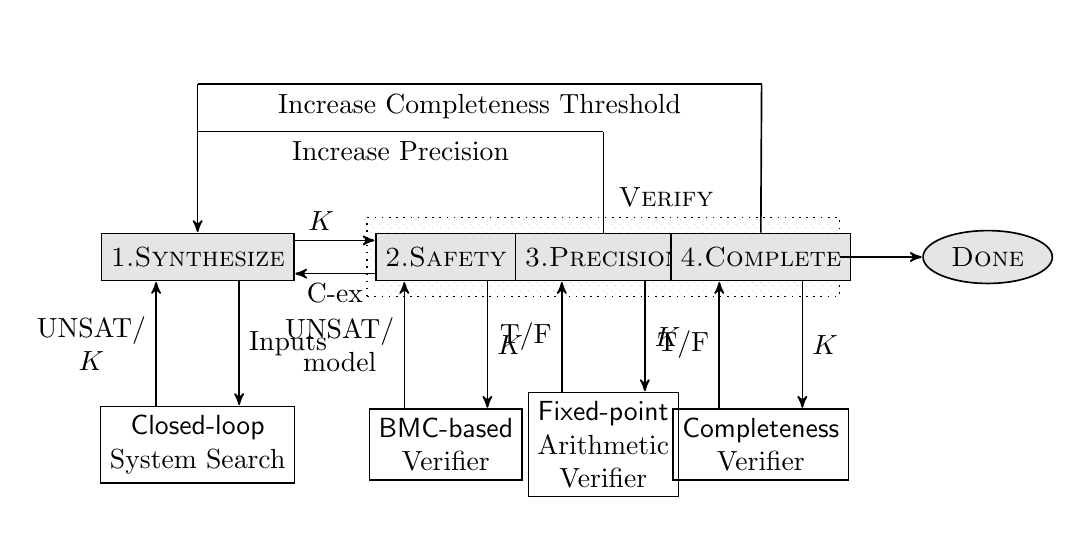
\begin{tikzpicture}[scale=0.3,->,>=stealth',shorten >=.2pt,auto, semithick, initial text=, ampersand replacement=\&,]
  \matrix[nodes={draw, fill=none, shape=rectangle, minimum height=.2cm, minimum width=.2cm, align=center
},
          row sep=.6cm, column sep=.9cm] {
   \coordinate (aux1);
   \& \coordinate (aux2);
   \&;\\
   \coordinate (aux3);
   \& \coordinate (aux4);
   \&;\\
   \coordinate (aux5);
   \& \coordinate (aux6);
   \&;\\
   \node[minimum width=1.5cm, minimum height=0.6cm, fill=gray!20] (synth) {{\sc 1.Synthesize}};
   \&
   complexnode/.pic={ 
     \node[rectangle,draw,dotted,
	minimum width=6cm,
	minimum height=1cm,
        pattern=north west lines, pattern color=gray!20,
	label={\sc ~~~~~~~~~~~~Verify},] (verif) {};
     \node[minimum width=1cm, minimum height=0.6cm, fill=gray!20] (verif1) at ([xshift=-2cm]verif.center) {{\sc 2.Safety}};
     \node[minimum width=1cm, minimum height=0.6cm, fill=gray!20] (verif2) at ([xshift=0cm]verif.center) {{\sc 3.Precision}};
     \node[minimum width=1cm, minimum height=0.6cm, fill=gray!20] (verif3) at ([xshift=2cm]verif.center) {{\sc 4.Complete}};
     %\node[minimum width=1cm, minimum height=0.6cm, fill=gray!20] (verif4) at ([xshift=3.1cm]verif.center) {{\sc 5.Sampling}};
   } 
   \& \node[ellipse, fill=gray!20] (done) {{\sc Done}};\\
   \& \\
   \node[minimum height=0cm] (gp) {\sf Closed-loop \\ System Search};
   \&
   complexnode/.pic={ 
     \coordinate (aux);
   \node (bmc) at ([xshift=-2cm]aux.center) {\sf BMC-based \\Verifier};
   \node (fp)  at ([xshift=0cm]aux.center) {\sf Fixed-point \\ Arithmetic\\Verifier};
   \node (sv)  at ([xshift=2cm]aux.center) {\sf Completeness\\Verifier};
   %\node (cv)  at ([xshift=3.1cm]aux.center) {\sf Sampling\\Verifier};
   }   
    \\
  };

   \path
    ([yshift=2em]synth.east) edge node[xshift=-0.5em,align=center] {$K$} ([yshift=2em]verif1.west)
    ([yshift=-2em]verif1.west) edge node {C-ex} ([yshift=-2em]synth.east)
    ([xshift=-5em]fp.north) edge node[align=center]  {T/F} ([xshift=-5em]verif2.south)
    ([xshift=-5em]sv.north) edge node[align=center]  {T/F} ([xshift=-5em]verif3.south)
    %([xshift=-5em]cv.north) edge node[align=center]  {T/F} ([xshift=-5em]verif4.south)
    ([xshift=5em]verif1.south) edge node[align=center] {$K$} ([xshift=5em]bmc.north)
    ([xshift=5em]verif2.south) edge node[align=center] {$K$} ([xshift=5em]fp.north)
    ([xshift=5em]verif3.south) edge node[align=center] {$K$} ([xshift=5em]sv.north)
    %([xshift=5em]verif4.south) edge node[align=center] {$K$} ([xshift=5em]cv.north)
    ([xshift=-5em]bmc.north) edge node[align=center]  {UNSAT/\\model} ([xshift=-5em]verif1.south)
    (verif) edge node {} (done)
    ([xshift=5em]synth.south) edge node[align=center] {Inputs} ([xshift=5em]gp.north)
    ([xshift=-5em]gp.north) edge node[align=center] {UNSAT/\\$K$} ([xshift=-5em]synth.south)
    (aux3) edge (synth.north);
   \path[-]
   (verif2.north) edge node[align=center] {} ([xshift=0cm]aux6)
   ([xshift=0cm]aux6) edge node[align=center] {Increase Precision} (aux5)
   (verif3.north) edge node[align=center] {} ([xshift=6.7cm]aux4)
   ([xshift=6.7cm]aux4) edge node[align=center] {Increase Completeness Threshold} (aux3);
   %(verif4.north) edge node[align=center] {} ([xshift=10.5cm]aux2)
   %([xshift=10.5cm]aux2) edge node[align=center] {Increase Sampling Rate} (aux1);

 \end{tikzpicture}
}}
\caption{CEGIS with multi-staged verification.}
\label{fig:CEGIS-precision-increment}
\end{figure}

%\subsubsection{Controller synthesis}

An overview of the controller synthesis is given in
Fig.~\ref{fig:CEGIS-precision-increment}.  One important observation is
that, for this approach, we verify and synthesize a controller over $k$ time
steps.  We~then compute a completeness threshold, $\overline{k}$, for this
controller, and verify correctness for $\overline{k}$ time steps. 
Essentially, $\overline{k}$ is the number of iterations required to
sufficiently unwind the closed-loop state-space system such that the
boundaries are not violated for any $k{>}\overline{k}$ (i.e., it is
sufficient to unwind the closed-loop state-space system up to $\overline{k}$
in order to ensure that $\phi_\mathit{safety}$ holds).

\medskip

Next, we describe the different phases in Fig.~\ref{fig:CEGIS-precision-increment}
(blocks 1 to 4) in detail.

%\todo{please eventually itemize next}
\begin{enumerate}

\item The inductive synthesis phase (i.e., {\sc synthesize}) uses BMC to
compute a candidate solution $K$ that satisfies both the stability criteria
(Sec.~\ref{ssec:stability}) and the safety specification
(Sec.~\ref{ssec:safety}).  To synthesize a controller that satisfies the
stability criteria, we require that a computed characteristic polynomial
satisfies Jury's criteria.  The details of this calculation can be found in
the Appendix.

 %\todo{unclear next: it seems like to select a single initial state here, rather than considering the set thereof - clarify. also, clarify relationship btw k and soundness. }

Regarding the second requirement, we synthesize a safe controller by
unwinding the transition system $k$ steps and by picking a controller $K$
and a single initial state, such that the states at each step do not violate
the safety criteria.  That is, we ask the bounded model checker if there
exists a $K$ that is safe for at least one $x_0$ in our set of all possible
initial states.  This is sound if the current $k$ is below the completeness
threshold, which we assume to be true in the {\sc synthesize} phase.  We
also assume some precision $\langle I_p,F_p\rangle$ for the plant and a
sampling rate.  The checks that these assumptions hold are performed by
subsequent {\sc verify} stages.

%\begin{algorithm}[]
%\scriptsize
%\begin{algorithmic}[1]
%\Function{$stabilityCheck()$}{}
%  \State computecharPoly($A_d - B_dK$)
%  \State assert(Jury's criteria hold)
  %\State Return $K$
%\EndFunction
%\end{algorithmic}
%\label{alg:stabilitycheck}
%\end{algorithm}


\begin{algorithm}[]
\scriptsize
\begin{algorithmic}[1]
\Function{$\mathit{safetyCheck}()$}{}
\State assert($ \underline{u}  \leq u \leq \overline{u}$)
 \State set $x_0$ to be a vertex state, e.g., $[\underline{x_0},\underline{x_0}]$	
\For {($c=0; c < 2^\mathit{Num\_States}; c++$)}
  %\State assert($ \underline{x_0}  \leq x_0 \leq \overline{x_0}$)
	\While{$i=0; i< k; i++$}
		%\State $u = (\langle I_p,F_p\rangle)((\langle I_c,F_c\rangle)K * (\langle I_c,F_c\rangle) x)$
		\State $u = (plant\_typet)((controller\_typet)K * (controller\_typet) x)$
		\State $x = A * x + B * u$
		\State assert($\underline{x} \leq x \leq \overline{x}$ )
  	\EndWhile
  	\State set $x_0$ to be a new vertex state
  	\EndFor
  %\State Return $K$
\EndFunction
\end{algorithmic}
\label{alg:safetycheck}
\end{algorithm}

\item The first {\sc verify} stage, {\sc safety}, checks that candidate
solution $K$, which we synthesized to be safe for at least one initial state, is safe for \emph{all} possible initial states, i.e., does not reach an unsafe
state within $k$ steps where we assume $k$ to be under the completeness threshold. 
After unwinding the transition system corresponding to the previously synthesized controller
$k$ steps, we check that the safety specification holds for any initial state. 

This is relatively computationally expensive if the bounds on the
allowed initial states are large.  However, we can show that, if the
controller is safe for each of the corner cases of our hypercube of
allowed initial states, it is safe for any initial state in the
hypercube. Thus we only need to check $2^n$ initial states, where $n$
is the dimension of the state space (number of continuous variables). 

To argue for this sufficient check, 
consider the set of initial states, $X_0$, which we assume to be convex since it's a hypercube. 
Name $v_i$ its vertexes, where $i=1,\ldots, 2^n$.  
Thus any point $x \in X_0$ can be expressed by convexity as $x = \sum_{i=1}^{2^n} \alpha_i v_i$, 
where $\sum_{i=1}^{2^n} \alpha_i =1$. Then if $x_0=x$, we obtain 
\begin{align*}
x_k   &= (A_d - B_d K)^k x = (A_d - B_d K)^k \sum_{i=1}^{2^n} \alpha_i v_i 
      = \sum_{i=1}^{2^n} \alpha_i (A_d - B_d K)^k v_i = \sum_{i=1}^{2^n} \alpha_i x_k^i, 
 \end{align*}     
%
where $x_k^i$ denotes the trajectories obtained from the single vertex
$v_i$.  We~conclude that any $k$-step trajectory is encompassed, within a
convex set, by those generated from the vertices.

\item The second {\sc verify} stage, {\sc precision}, 
 restores soundness with respect to the plant's precision
by using interval arithmetic \cite{moore1966interval} to validate the 
operations performed by the previous stage. 

\item The third {\sc verify} stage, {\sc complete}, checks that the current
$k$ is large enough to ensure safety for any $k'{>}k$.  Here, we compute the
completeness threshold $\overline{k}$ for the current candidate $K$ and
check that $k{\leq}\overline{k}$.  This is done according to the following
argument, illustrated in Fig.~\ref{fig:ct}.

A stable control system is known to have converging dynamics.  Assume the
closed-loop matrix eigenvalues are not repeated (which is sensible to do,
since we select them).  The distance of the trajectory from the reference
point (origin) decreases over time within subspaces related to real-valued
eigenvalues; however, this in general not the case when dealing with complex
eigenvalues.  Consider the closed-loop matrix, which updates the states
every discrete time step, and select the eigenvalue $\vartheta$ with
smallest (non-trivial) imaginary value.  At every consecutive time steps
$kT_s, (k+1)T_s$, the dynamics projected on the corresponding eigenspace
rotate of $\vartheta T_s$ radiants.  So taking $k{\leq}\overline{k}$ as the
ceiling of $\frac{2\pi}{\vartheta T_s}$, after $k{\leq}\overline{k}$ steps
we have completed a full rotation, which results in a point closer to the
origin, and it is the completeness threshold.

\begin{figure*}[t]
\centering
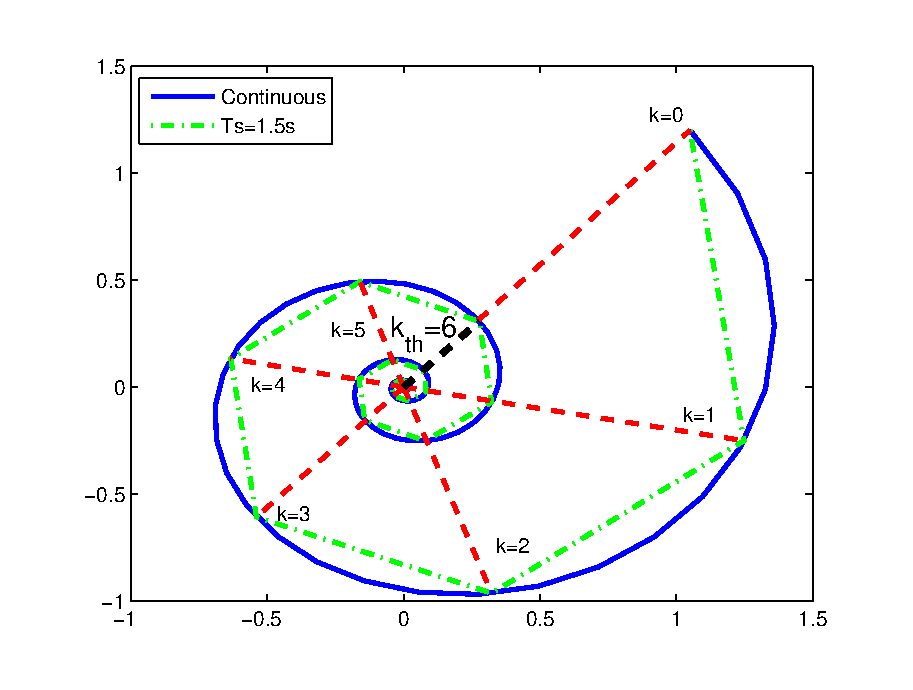
\includegraphics[width=0.6\textwidth]{ct.eps}
\vspace{0.1cm}
\caption{Completeness threshold for multi-staged verification}
\label{fig:ct}
\end{figure*}

\end{enumerate}

\subsubsection{Illustrative Example} \label{sec:running-ex}

We illustrate our approach with an example,
extracted from the literature~\cite{Franklin15}.
%
We start with a candidate solution with all coefficients zero, $K=[0
  \ 0 \ 0]^T$, and a precision of $I_p=13$, $F_p=3$.  In the first
{\sc verify} stage, the {\sc safety} check finds the counterexample
%
$ x_0 = [-0.5 \ 0.5 \ 0.5] $.
%
After adding the new counterexample to its sets of {\sc inputs}, {\sc
  synthesize} finds the candidate solution $K=[0 \ 0
  \ 0.00048828125]^T$, which prompts the {\sc safety} verifier to
return $x_0=[-0.5 -0.5 -0.5]$ as the new counterexample.

In the subsequent iteration, the synthesizer is unable to find further 
suitable candidates and it returns UNSAT, meaning that the current precision is
insufficient.  Consequently, we increase the precision to $I_p=17$,
$F_p=7$.
%
Since the previous counterexamples were obtained at lower precision,
we remove them from the set of counterexamples.  Back in the {\sc
  synthesize} phase, we re-start the process with a candidate solution
with all coefficients $0$.  Next, the {\sc safety} verification stage
provides the first counterexample at higher precision, $x_0=[-0.5
  \ 0.5 \ 0.5]$ and {\sc synthesize} finds $K=[0 \ 0.01171875
  \ 0.015625]^T$ as a candidate that eliminates this counterexample.
However, this candidate triggers the counterexample
$x_0=[0.5\ -0.5\ -0.5]$ found again by the {\sc safety} verification
stage.  In the next iteration, we get the candidate $K=[0 \ 0
  \ -0.015625]$, followed by the counterexample $x_0 = [0.5 \ 0.5
  \ 0.5]$. Finally, {\sc synthesize} finds the candidate $K=[0.01171875
  \ -0.013671875 \ -0.013671875]^T$, which is validated as a final
solution by all verification stages.

%+++++++++++++++++++++++++++++++++++++++++++++++++++++++++++++++++++++++++++++++
\subsection{Abstraction-based CEGIS}
\label{sec:CEGIS-abstraction-refinement}
%+++++++++++++++++++++++++++++++++++++++++++++++++++++++++++++++++++++++++++++++


%\begin{itemize}
%\item[1.]

  The naive approach described in Sec.~\ref{sec:CEGIS-precision-incrementation}
  %uses a multi-staged verification phase and performs solution generalization based on
%the plant precision, the number of loop unrollings, 
  %and the sampling rate. Essentially, it
  synthesizes a controller for an individual initial state
and input with a bounded time horizon and, subsequently, it generalizes it to all reachable states,
inputs, and time horizons during the verification phase.
Essentially, this approach relies on the explicit
simulation over a bounded time horizon of individual states that form
part of an uncountable space and tries to generalize it for an
infinite space over an infinite time horizon.

  %% solution over all times by refining the number of witnesses.  
  %% In order to perform the safety check, this approach uses abstract acceleration
  %% \cite{cattaruzza2015unbounded} to compute the controller's set of states. 
  %% \todo{clarify: what is the ``set of states'' of the controller? }
%\end{itemize}

%% The verification of a hybrid continuous/discrete system over an
%% unbounded time, requires the non-deterministic simulation of an
%% infinite set of states, which is undecidable.


%% Our naive approach
%% creates an abstraction of the system by establishing bounds on the
%% error between such a system and a discrete-time/continuous-space
%% model.  This model is still however, quite complex, hard to verify,
%% and many of the states involved are inconsequential to the safety
%% specification.

Conversely, in this section, 
we  find a controller for a continuous initial set of states and set of inputs, 
  over an abstraction of the continuous dynamics that conforms to
  witness proofs at specific times. %% It further generalizes the
  Moreover, this approach uses abstraction refinement enabling us to 
  always start with a very simple description regardless of the complexity of the overall
dynamics, and only expand to more complex models when a solution
cannot be found.

  The CEGIS loop for this approach is illustrated in Fig.~\ref{fig:CEGARIS}.

% Now that we have explained the verification process, we may proceed to describe the synthesis procedure, which is illustrated in figure \ref{fig:CEGARIS}.
% Our model, rather than look at a bisimulation \todo{specific notion that has not been formally define - do not use} in discrete time, explores a much higher abstraction, 
% evaluating the unbounded time-continuous space reach tube as a set of inequalities that represent only the safety specification.
% We have also identified 
% the quantization noise as a bounded non-deterministic input.


\begin{enumerate}
\item 
  We start by doing some preprocessing:%%  that 
  %% can be computationally intensive and we don't want it to be part of the CEGIS loop.
% Let us recall the formulas used for single-input and single-output (SISO) systems 
  % in sections \ref{sec:reachable} and \ref{sec:observable}.
  \begin{enumerate}
\item Compute the characteristic polynomial of the matrix $(A_d-B_dK)$ as 
$P_a(z) = z^n+\sum_{i=1}^p{(a_i-k_i)z^{n-i}}$.
%%   A controllable system with quantization will have the following dynamics, where
%% we use underscript ``n'' to denote a noise term,
%% ``cf'' to denote Controllable Canonical Form,
%% $\nu_1$, $\nu_2$ are quantization errors
%% caused by the ADC and DAC conversions, respectively, 
%% and $\nu_3$ is the round-off error.
%% \todo{Why do we use $_t$ here?}
%% %
%% \begin{align}
%% \label{eq:observer_LTI_cf}
%% x_{k+1}=&\mat{A}_{t}x_k+\mat{B}_{t} r_k+\mat{B}_{n} (\nu_1 + \nu_2 + \nu_3)
%% \end{align}
%% \begin{align*}
%% \mat{A}_{t}=&\mat{T}\mat{A}_d\mat{T}^{-1}&
%% \mat{B}_{t}=&\mat{T}\mat{B}_d&
%% \mat{B}_{n}=&[1 \cdots 1]^T&
%% \mat{T}=&\mat{W}_{cf}\mat{W}^{-1}&
%% \end{align*}

%% \begin{align*}
%% \mat{A}_{t}=\mat{T}\mat{A}_d\mat{T}^{-1}=&\left[
%% \begin{array}{ccccc}
%% 0&1&0&\cdots&0\\
%% 0&0&1&\cdots&0\\
%% \vdots&\vdots&\vdots&\ddots&\vdots\\
%% 0&0&0&\cdots&1\\
%% k_n-a_n&k_{n-1}-a_{n-1}&k_{n-2}-a_{n-2}&\cdots&k_1-a_1
%% \end{array}\right]
%% \label{eq:cf_SISO_2}
%% \end{align*}


%% \begin{enumerate}
%% \item Calculate $\mat{T}$ as $\mat{W}_{cf}\mat{W}^{-1}$. %using equations \eqref{eq:rncf}\eqref{eq:rcf}\eqref{eq:to_cf}
%% \item Extract the characteristic polynomial of the above matrix:
%% %
%\begin{align*}
%$P_a = z^n+\sum_{i=1}^p{(a_i-k_i)z^{n-i}}$
%\end{align*}

\item Calculate the noise set $N$ from the quantizer resolutions and estimated round-off errors: %($\frac{q_1}{2},\frac{q_2}{2},q_3$)
%
$$N=\left \{ \nu_1+\nu_2+ \nu_3 : \nu_1 \in \left[-\frac{q_1}{2}\ \ \frac{q_1}{2}\right] 
\wedge \nu_2 \in \left[-\frac{q_2}{2}\ \ \frac{q_2}{2}\right]  \wedge \nu_3 \in \left[-q_3\ \ q_3\right]  \right \}\nonumber$$
%
where  $q_1$ is the error introduced by the truncation by the ADC, $q_2$ is
the error introduced by the DAC and $q_3$ is the maximum truncation and
rounding error in $u_k=-K \cdot \mathcal{F}_{\langle I_c,F_c \rangle}(x_k)$ as
discussed in Section~\ref{sec:numeric_rep}.  More details on how to model
quantization as noise are given in
Appendix~\ref{appendix:quantization-noise}.

\item Calculate a set of initial bounds on $K$, $\phi_\mathit{init}^{K}$,
based on the input constraints.  Note that these bounds will be used by the
{\sc synthesize} phase to reduce the size of the solution space. 
%
$$(\phi_\mathit{init} \wedge \phi_\mathit{input} \wedge u_k=-K x_k)
\Rightarrow \phi_\mathit{init}^{K}$$

\end{enumerate}
\item In the {\sc synthesize} phase, we synthesize a candidate controller
%We begin with a minimum set of linear inequalities describing the constraints caused by the input and the initial state during a single iteration, in addition to a stability 
% specification defined by Jury's 
%criteria. %, and try to synthesise a controller that meets these specs.
% For a stabilized closed-loop, which is necessary for our safety property, we need
% these roots to remain within the unit circle, which we verify using Jury's criteria.
% Notice that in our polynomials $c_0=1$ and we only use reals.
% Once we have established convergence, we may examine the 
% safety specification $\phi_{safety}$.
  $K \in \mathbb{R}\langle I_c,F_c\rangle^n$ that satisfies
  $\phi_\mathit{stability} \wedge \phi_\mathit{safety} \wedge \phi_\mathit{init}^{K}$ by invoking a SAT solver.
%%   We obtain it by solving the SAT formula 
%% $$\mathcal{J}_K=\mathcal{J}\langle I,F \rangle (P_{a-k},\mat{T})\wedge \phi_{safety}$$ 
%% that satisfies the input constraint and Jury's criteria for 
%% $P_{a-k}=z^n+\sum_{i=1}^n (a_i-k_i) z^{n-i} : k_i \in \mat{K} \wedge \tilde{\mat{K}}=\mat{K}\mat{T}$,
%% where $\mathcal{J}\langle I,F \rangle (P,\mat{T})$ is a program describing Jury's method.
If there is no candidate solution we return UNSAT and exit the loop.
\item Once we have a candidate solution, we perform a safety verification % If this step fails, we find a counterexample iteration and initial state and create a new constraint to refine our abstraction.
  %
  of the 
  %consisting of evaluating the
  progression of the system from $\phi_\mathit{init}$ over time,
$x_{k+1} \models \phi_\mathit{safety}$. %% For this purpose we require 
%% an initial set $\phi_{init}= x_0 \in [\underline{x_0} \ \overline{x_0}]$ 
%% from which the system progresses.
% Obviously, this set $x_0$ 
% must satisfy the specification; otherwise, the system will be unsafe to begin with.
% We accept a specification in the form $\mat{E}\mat{T}x_0<\mat{f}$. 
% The presence of $\mat{T}$ is because this will typically be given in the original 
% state-space.
%% Next, we use abstract acceleration to get a second abstraction that 
  %% encompasses the accelerated continuous reach-tube over an unbounded time.
  In order to compute the progression of point $x_0$ at iteration $k$,
  we accelerate the dynamics of the closed-loop system and obtain:
  %we take the
  %the closed-loop model:
  %$x_{k+1}=\mat{A}_{t}x_k+\mat{B}_{n} (\nu_1 + \nu_2 + \nu_3)$
  %and accelerate it to:
%
\begin{align}
%\label{eq:acc_observer_LTI_cf}
x=&(A_d-B_dK)^kx_0
%+\sum_{i=0}^{k-1} \mat{A}_t^i \mat{B}_{t} r_i
+\sum_{i=0}^{k-1} (A_d-B_dK)^i B_{n}(\nu_1+\nu_2+\nu_3) : B_n= [1\ 1 \cdots \ 1 ]^T
\end{align}
%
As this still requires us to verify the system for every $k$ up to infinity,
we use abstract acceleration again to obtain the reach-tube, i.e., the set
of all reachable states at all times given an initial set
$\phi_\mathit{init}$:
%
\begin{align}
\label{eq:aa_observer_LTI_cf}
\hat{X}^\#
=&\mathcal{A} X_0 + \mathcal{B}_{n} N\\
X_0 =&\left \{x : x \models \phi_\mathit{init} \right\}\nonumber
\end{align}
%
where $\mathcal{A}=\bigcup_{k=1}^\infty (A_d-B_dK)t^k,
\mathcal{B}_{n}=\bigcup_{k=1}^\infty \sum_{i=0}^k(A_d-B_dK)^iB_{n}$ are
abstract matrices for the closed-loop system~\cite{cattaruzza2015unbounded},
whereas the set $N$ is non-deterministically chosen.

We next evaluate $\hat{X}^\# \models \phi_\mathit{safety}$.  If the
verification holds we have a solution, and exit the loop.  Otherwise, we
find a counterexample iteration $k$ and corresponding initial point $x_0$
for which the property does not hold, which we use to locally refine the
abstraction.  When the abstraction cannot be further refined, we provide
them to the {\sc abstract} phase.
%
%\todo{we should have a better argument here.}
%\end{enumerate} 
\item If we reach the {\sc abstract} phase, it means that the candidate solution is not valid,
  in which case we must refine the abstraction used by the synthesizer.
\begin{enumerate}
\item Find the constraints that invalidate the property
 as a set of counterexamples for the eigenvalues, which we define as $\phi_\Lambda$. This is a constraint in the spectrum i.e., transfer function) of the closed loop dynamics. 
\item We use $\phi_\Lambda$ to
  further constrain the characteristic polynomial  
$z^n+\sum_{i=1}^n(a_i-k_i)z^{n-i}=\prod_{i=1}^n (z-\lambda_i) : |\lambda_i|<1 \wedge \lambda_i \models \phi_{\Lambda}$. These constraints correspond to specific iterations for which the system may be unsafe.
\item Pass the refined abstraction $\phi(K)$ with the new constraints and the list of iterations $\vec{k}$ to the {\sc synthesize} phase.
  %, as well as a counterexample plant coefficients ($P_a$) and repeat the loop again. 
\end{enumerate} 
\end{enumerate}

\subsubsection{Illustrative Example}
%
Let us consider the Helicopter example in Table
\ref{table:State-space-benchmarks} with discretized dynamics
%
$$A_d = \left[\begin{array}{ccc}2.6207&-1.1793&0.65705\\2&0&0\\0&0.5&0\end{array}\right],
\quad B_d = \left [\begin{array}{c}8\\0\\0\end{array}\right]$$
%
Using the initial state bounds $\underline{x_{0}}=-0.9$ and
$\overline{x_{0}}=0.9$, the input bounds $\underline{u}=-10$ and
$\overline{u}=10$, and safety specifications $\underline{x_{i}}=-0.92$ and
$\overline{x_{i}}=0.92$, the {\sc synthesize} phase in
Fig.~\ref{fig:CEGARIS} synthesizes an initial candidate controller
$K=[\begin{array}{ccc}0.24609375&-0.125&0.1484375\end{array}]$.
Although this candidate is stable, the {\sc verify} phase finds it to be
unsafe and returns a list of iterations with an example initial state that
fails the safety specification {\footnotesize $(k,x_0) {\in}
\{ (2, [\begin{array}{ccc}0.9&-0.9&0.9\end{array}]),\allowbreak (3,
[\begin{array}{ccc}0.9&-0.9&-0.9\end{array}])\}$}.  This allows the {\sc
abstract} phase to create a new safety specification that considers these
iterations for these initial states to constrain the solution space.  This
refinement allows {\sc synthesize} to find a controller {\footnotesize
$K=[\begin{array}{ccc}0.23828125&-0.17578125&0.109375\end{array}]$}, which
this time passes the verification phase, resulting in a safe system.

%% Note that the abstraction refinement is a constraint on the proposed model which can increase or decrease the parameter space at any time, whereas the concrete counterexample passed to the synthesizer is monotonically decreasing. The former improves the speed of the tool, whereas the second ensures convergence.

\begin{figure}
\centering
{\scriptsize
\hspace*{-1cm}
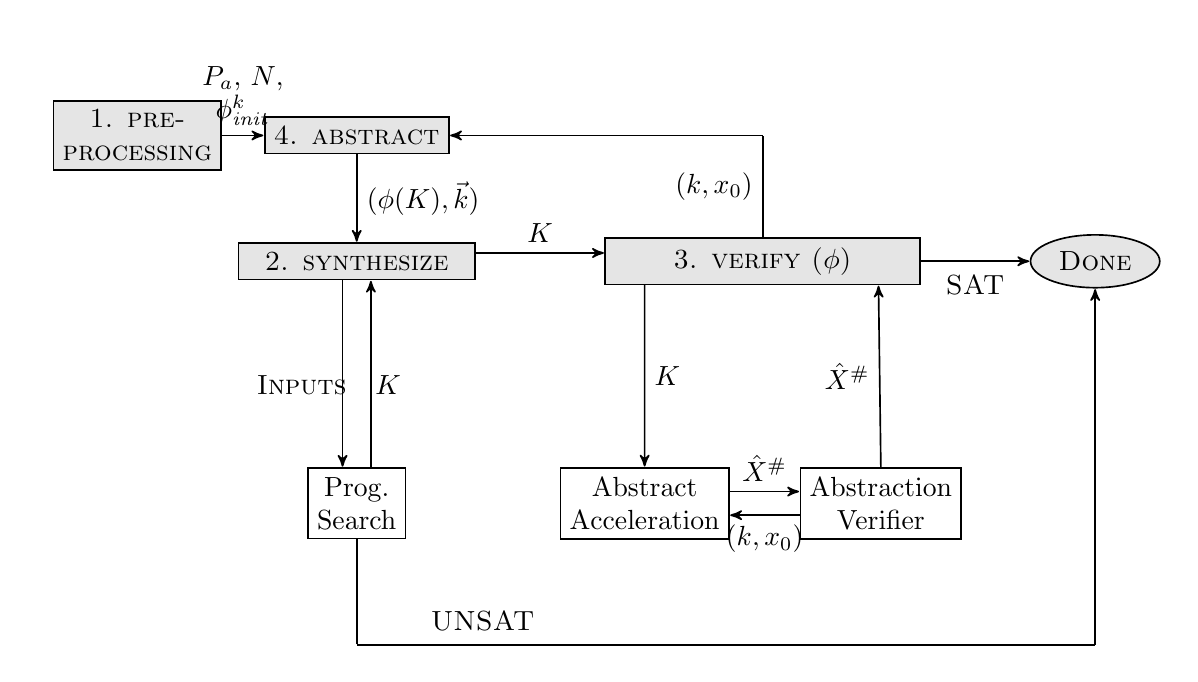
\begin{tikzpicture}[scale=0.3,->,>=stealth',shorten >=.2pt,auto, semithick, ampersand replacement=\&,]
  \matrix[nodes={draw, fill=none, shape=rectangle, minimum height=.2cm, minimum width=.2cm, align=center},row sep=.8cm, column sep=.2cm] {
   \coordinate (aux1);
   \& \coordinate (aux2);
   \& ;\\
   \&\node[fill=gray!20,align=center] (pre) {{\sc 1. pre-}\\{\sc processing}};
   \& \node[fill=gray!20,align=center] (abstract) {\sc 4. abstract};
   \& \coordinate (aux); \\ % \node[fill=yellow!20,align=center] (counter) {\sc counterexample};\\
   \& 
   \& \node[fill=gray!20,align=center, minimum width=3cm] (synth) {\sc 2. synthesize};
       %\node[draw=none] (KL) at ([xshift=2.5cm,yshift=-.25cm]synth)  {\sc $\mat{K},\mat{L}$};
       %\node[draw=none] (NKL) at ([xshift=2cm,yshift=1cm]synth)  {\sc $P_a$};
   \& \node[fill=gray!20,align=center, minimum width=4cm] (verify) {\sc 3. verify ($\phi$)};
       %\node[draw=none] (VUNS) at ([xshift=.6cm,yshift=1cm]verify)  {\sc SAT};
       \node[draw=none] (SAT) at ([xshift=2.7cm,yshift=-.3cm]verify)  {\sc SAT};
   \& \node[ellipse, fill=gray!20] (done) {{\sc Done}};\\
   \&
   \& complexnode/.pic={
     \coordinate (auxsynth);
     \node[draw,rectangle,align=center] (KSAT) at ([xshift=0cm]auxsynth.center) {Prog.\\Search};
     \node[draw=none] (SATK) at ([xshift=-.7cm,yshift=1.5cm]KSAT)  {{\sc Inputs}};
     \node[draw=none] (K) at ([xshift=.4cm,yshift=1.5cm]KSAT)  {$K$};
    }
   \& complexnode/.pic={
     \coordinate (AA);
     \node[draw,rectangle,align=center] (AAV) at ([xshift=-1.5cm]AA.center) {Abstract\\Acceleration};
     \node[draw,rectangle,align=center] (AAC) at ([xshift=1.5cm]AA.center) {Abstraction \\ Verifier};
    }\\
   \&
   \& complexnode/.pic={
     \coordinate (UNSAT);
     \coordinate (KUNSAT)  at ([xshift=0cm]UNSAT.center);
     \node[draw=none] (UNSATB) at ([xshift=1.6cm,yshift=.3cm]UNSAT)  {\sc UNSAT};
  }
  \& \& \coordinate (FAIL);\\
  };
  \path
    (pre.east) edge node[align=center] {$P_a$, $N$,\\ $\phi_\mathit{init}^k$} (abstract.west)
    (abstract.south) edge node{$(\phi(K), \vec{k})$} (synth.north)
    %([yshift=2em]synth.east) edge node {Candidate} ([yshift=2em]verif.west)
    %([yshift=-2em]verif.west) edge node {New input} ([yshift=-2em]synth.east)
    %([yshift=2em]synth.east) edge node[xshift=-0.7em] {Candidate} ([yshift=2em]verif.west)
    %([yshift=-2em]verif.west) edge node[xshift=-0.7em] {New input} ([yshift=-2em]synth.east)
    ([yshift=1em]synth.east) edge node {$K$} ([yshift=1em]verify.west)
    %([yshift=-1em]verify.west) edge node {$P_a$} ([yshift=-1em]synth.east)
    (aux) edge (abstract.east) 
    (verify.east) edge (done.west);
  \path
    ([xshift=+.6cm]KSAT.north) edge ([xshift=0.6cm]synth.south) 
    ([xshift=-.6cm]synth.south) edge ([xshift=-.6cm]KSAT.north)
    %(AAC) edge[bend right] node[align=center] {$k$} (AAI.north)
    %([xshift=-4.9cm]verify.south) edge node[align=center] {$\mat{A},\mat{B}$\\$\phi$} (AAI.north)
    %(AAI.east) edge (AAV.west)
    ([yshift=.5cm]AAV.east) edge node{\sl $\hat{X}^\#$} ([yshift=.5cm]AAC.west)
    ([yshift=-.5cm]AAC.west) edge node{$(k,x_0)$} ([yshift=-.5cm]AAV.east)
    (AAC.north) edge node{\sl $\hat{X}^\#$} ([xshift=4.9cm]verify.south)
    %(AAC.west) edge (AB.west)
    %(verify.north) edge (counter.south)
    %(counter.west) edge (abstract.east)
    %(counter.south west) edge (synth.north east)
    (FAIL.north) edge (done.south)
    ([xshift=-5cm]verify.south) edge node{$K$} (AAV.north);
  \path[-] 
     (KSAT.south) edge (KUNSAT.north)
     (KUNSAT.east) edge (FAIL.west)
     (verify.north) edge node {$(k,x_0)$} (aux);
\end{tikzpicture}
}
\caption{Abstraction-based CEGIS.}
\label{fig:CEGARIS} 
\end{figure}

%-------------------------------
\section{Experimental Evaluation}
%-------------------------------

%-------------------------------
\subsection{Description of the Benchmarks}
\label{experimental-setup}
%-------------------------------

A set of state-space models for different classes of systems was extracted
from the literature~\cite{Franklin15, maglev, converters, CTMS} and employed
for validating our methodology.

\textit{DC Motor Rate} plants describes the angular velocity of a DC Motor, respectively. 
The \textit{Automotive Cruise System} plant represents the speed of a motor vehicle. 
The \textit{Helicopter Longitudinal Motion} plant provides the longitudinal motion model 
of a helicopter. 
The \textit{Inverted Pendulum} plant describes a pendulum model
with its center of mass above its pivot point. 
The \textit{Magnetic Suspension} plant provides a physical model for which 
a given object is suspended via magnetic field. 
The \textit{Magnetized Pointer} plant describes a physical model employed in analogue gauges 
and indicators that is rotated through interaction with magnetic fields.
The \textit{1/4 Car Suspension} plant presents a physical model that connects a car to its wheels 
and allows relative motion between both parts.
The \textit{Computer Tape Driver} plant describes a system to read and write data 
on a storage device in the computer.

Section~\ref{sec:BenchmarksforStateSpace} in the appendix summarizes all our
benchmarks, which are SISO models (Section~\ref{sec:preliminaries}).  The
Inverted Pendulum appears to be a two output system, but it was treated as
two SISO systems during the experiments.  For the sake of simplicity all the
state measurements are assumed available.  In practice, state estimators
should be designed in order to obtain an estimate of the states from the
single output.  Further work can include state observers synthesis.

All benchmarks were discretized with different sample times using 
the approach described in Appendix~\ref{sec:appendix:LTIbackground}. 
All experiments were performed considering $\underline{x_{i}}=-1$ and 
$\overline{x_{i}}=1$ and the inputs $u_{k}=0, \forall k>0$.
We have conducted the experimental evaluation on a 12-core 2.40\,GHz Intel
Xeon E5-2440 with 96\,GB of RAM and Linux OS.  We used the Linux
\emph{times} command to measure CPU time used for each benchmark.  The
runtime was limited to one hour per benchmark.

%-------------------------------
\subsection{Objectives}
%-------------------------------

Using the state-space models given in Section~\ref{experimental-setup}, 
our experimental evaluation aims to answer two research questions:
%
\begin{enumerate}

\item[RQ1] \textbf{(CEGIS)} do the multi-staged verification and abstraction-based
CEGIS generate a FWL digital controller in a reasonable amount of time?

\item[RQ2] \textbf{(sanity check)} are the synthesized controllers sound
and can their stability and safety be confirmed outside of our model?

\end{enumerate}


%-------------------------------
\subsection{Results}
%-------------------------------

We give the run-times required to synthesize a stable controller for each
benchmark in Table~\ref{tab:results}.  Here \textit{Benchmark} is the name
of the respective benchmark, $\mathcal{F}_{\langle I_p,F_p \rangle}$ is the
fixed-point precision used to model the plant, while \textit{Time} is the
total time required to synthesize a stable controller for the given plant,
for CEGIS with multi-staged verification as well as abstraction-based CEGIS. 
The precision for the controller, $\mathcal{F}_{\langle I_c,F_c \rangle}$,
is always chosen to be $I_c = 8, F_c = 8$.

For the majority of our benchmarks, we observe that the abstraction-based
back-end is faster than the basic multi-staged verification approach. 
However, it fails to find solutions to three benchmarks, as compared to two
with the multi-staged back-end, where the numbers given in the
discretization matrices are too small.  In direct comparison, the
abstraction-based approach is on average able to find a solution in
approximately 35\% of the time required using the multi-staged back-end, and
has a median run-time 1.15\,s, which is seven times smaller than the
multi-staged approach.  The two back-ends complement each other in benchmark
coverage and together solve all benchmarks in the set.

\begin{table}
\centering
%\scriptsize
\begin{tabular}{| c | l | c | r | c | r |}
%
\hline
\# & \multicolumn{1}{|c|}{Benchmark}  & \multicolumn{2}{|c|}{Multi-staged}                 & \multicolumn{2}{|c|}{Abstraction} \\
   &                                  & \multicolumn{1}{|c|}{$\mathcal{F}_{\langle I_p,F_p \rangle}$} & \multicolumn{1}{|c|}{Time} & \multicolumn{1}{|c|}{$\mathcal{F}_{\langle I_p,F_p \rangle}$} & \multicolumn{1}{|c|}{Time} \\\hline
1  & Cruise Control      & 8,16   & 6.88\,s & 16,16  & 241    \\
2  & DC Motor            & 8,16   & 8.10\,s & 20,20  & 5376   \\
3  & Helicopter          & \xmark & \xmark  & 16,16  & 2120   \\
4  & Inverted Pendulum   & 8,16   & 7.81\,s & 16,16  & 387    \\
5  & Magnetic Pointer    & \xmark & \xmark  & 28,28  & 132845 \\
6  & Magnetic Suspension & 12,20  & 8.73\,s & 32,32  & 7854   \\
7  & Pendulum            & 8,16   & 9.01\,s & 20,20  & 1150   \\
8  & Suspension          & 12,20  &49.41\,s & \xmark & \xmark \\
9  & Tape Driver         & 8,16   & 9.18\,s & \xmark & \xmark \\
10 & Satellite           & 8,16   & 8.98\,s & \xmark & \xmark \\\hline
%
\end{tabular}
\caption{Experimental results\label{tab:results}}
\end{table}

The median run-time for our benchmark set is 7.9\,s.  Overall, the average
synthesis time amounts to approximately 17.2\,s.  We consider these times
short enough to be of practical use to control engineers, and thus affirm
RQ1.

There are several cases for which the system may fail to find a controller. 
For the naive approach, the completeness threshold may be too large, thus
causing a timeout.  On the other hand, the abstraction-based approach may
require a very precise abstraction, resulting in too many refinements and,
consequently, a timeout.  Yet another source of incompleteness is the
inability of the {\sc synthesize} phase to use a large enough precision for
the plant model in a given problem.

The synthesized controllers were confirmed to be stable outside of our model
representation using MATLAB, positively answering RQ2.  A~link to the full
experimental environment, including scripts to reproduce the results, all
benchmarks and the tool, is provided in the
footnote.\footnote{\url{https://drive.google.com/open?id=0ByIexo3Z5N91eDludEdWdWxfV1E}}


%-------------------------------
\subsection{Threats to validity}
%-------------------------------

\textit{Benchmark selection:} We report an assessment of both our approaches
over a diverse set of real-world benchmarks.  Nevertheless, this set of
benchmarks is limited within the scope of this paper and the performance may
not generalize to other benchmarks.\\
%
\textit{Plant precision and discretization heuristic:} Our algorithm to
select suitable FWL word widths to model the plant behavior employs a
heuristic based on user-provided controller word-width specifications.  For
the first approach, where we may need to increase the precision of the time
discretization, we select the time steps for the discretizations on a
similar basis.  This works sufficiently well for our benchmarks, but
performance may suffer in some cases, for example if the completeness
threshold is high.\\
%
\textit{Abstraction on other properties:} The performance gain from abstract
acceleration may not hold for more complex properties than safety, for
instance ``eventually always reaches a certain safe set''.

%-------------------------------
\section{Conclusion}
%-------------------------------

We have presented two automated approaches to synthesize digital
state-feedback controllers that ensure both stability and safety over the
state-space representation.  The first approach relies on explicit unfolding
of the closed-loop model dynamics up to a completeness threshold, whilst the
second one applies abstraction refinement and acceleration to increase speed
whilst retaining soundness.
%
Both approaches are novel within the control literature: they give a fully
automated synthesis method that is algorithmically and numerically sound,
considering various error sources in the implementation of the digital
control algorithm and in the computational modeling of plant dynamics.
%
Our experimental results show that both approaches are able to synthesize
stable controllers for most benchmarks within a reasonable amount of time
fully automatically.  In particular, both approaches complement each other
and together solve all benchmarks, which have been derived from the control
literature.

Future work will focus the extension of these approaches to the
continuous-time case, to models with output-based control architectures
(hinging on the use of observers), and to considering performance
requirements (alongside safety) in the synthesis of digital controllers.

\newpage

\bibliographystyle{abbrv}
\bibliography{paper}  
%\begin{thebibliography}{4}
%\end{thebibliography}

\newpage
\appendix
%-------------------------------
\section{Stability of closed-loop models}
\label{sec:appendix-stability}
%-------------------------------

%\addtodo{[Here discuss Jury criterium for DISCRETE-TIME models - a simplified version of the first part of what is now in Section \ref{sec:cof_verification} (with no quantization noises yet).]}  

%-------------------------------
\subsection{Encoding of Jury's criterion}
%-------------------------------

For a closed-loop system as~\eqref{eq:closedloopss}, 
the characteristic polynomial $P(z)$ should be computed as follows:
%
\begin{equation}
P(z)= \det( z I_{n} - A_d + B_d K ) \,,
\end{equation}
%
where $I_{n}$ is the $n$-th order identity matrix. 

Jury's criterion provides necessary and sufficient conditions for the
eigenvalues to be within the unit circle and, consequently, for the system
is stable~\cite{fadali}.  Given a polynomial $P(z)$ of the form
%
$$
P(z) = a_{0}z^{N} + a_{1}z^{N-1} + ... a_{N-1}z + a_{N} = 0, \;\; a_{0}\neq 0 \,,
$$
%
Jury's criterion explores solely the coefficients
$a_{0},a_{1},\ldots,a_{N-1}$ of $P(z)$ for checking stability, which we
capture as property $\phi_\mathit{stability}$, as detailed below.

This study limits itself to explain the encoding of Jury's criterion for
formal synthesis.  For the stability test procedure, the following matrix
$M=[m_{ij}]_{(2N-2)\times N}$ is built from the coefficients of $P(z)$:
%
$$
M=\left[
\begin{matrix}
  V^{(0)} \\
  V^{(1)} \\
  \vdots \\
  V^{(N-2)}
 \end{matrix}
\right]\mbox{,}
$$
\noindent where $V^{(k)}=[v^{(k)}_{ij}]_{2\times N}$ is such that
$$
v^{(0)}_{ij}=\begin{cases} 
a_{j-1}, & \mbox{if } i=1 \\   v^{(0)}_{(1)(N-j+1)}, & \mbox{if } i=2 
\end{cases}\mbox{, and} 
$$
$$
v^{(k)}_{ij}=\begin{cases} 
0, & \mbox{if } j>n-k\\
v^{(k-1)}_{1j}-v^{(k-1)}_{2j}\cdot\frac{v^{(k-1)}_{11}}{v^{(k-1)}_{21}}, & \mbox{if } j\leq n-k  \mbox{ and } i=1 \\
v^{(k)}_{(1)(N-j+1)}, & \mbox{if } j\leq n-k \mbox{ and } i=2 \\
\end{cases} \mbox{,}
$$
\noindent where $k\in\mathbb{Z}$, such that $0<k<N-2$. $P(z)$ is the 
characteristic polynomial of a stable system if and only if the following 
four propositions hold:
\begin{itemize}
\item $R_{1}$: $P(1)>0$;
\item $R_{2}$: $(-1)^{N}P(-1)>0$;
\item $R_{3}$: $\vert{a_{0}}\vert <a_{N}$;
\item $R_{4}$: $m_{11}>0\iff (m_{31}>0)\wedge (m_{51}>0)\wedge \ldots \wedge (m_{(2N-3)(1)}>0)$.
\end{itemize}
%
The stability property $\phi_\mathit{stability}$ is encoded as the following formula:
$$
\phi_\mathit{stability}\iff \ (R_{1} \wedge R_{2} \wedge R_{3} \wedge R_{4}).
$$

%-------------------------------
\subsection{Stability of Closed-loop Systems with Fixed-point Controller Error}
%-------------------------------

The proof above relies on the fact that the relationship between states and
next states is defined by $x_{k+1} = (A_d - B_dK) \cdot x_k$, all computed
at infinite precision.  When we employ a FWL digital controller, the
operation becomes:
%
\begin{align*}
x_{k+1} &= A_d \cdot x_{k} -(\mathcal{F}_{\langle I_c,F_c \rangle}(K)\cdot\mathcal{F}_{\langle I_c,F_c \rangle}(x_{k})).  \\
x_{k+1} &= (A_d  - B_dK) \cdot x_k + B_dK\delta
%\\ x_{k+1}&=A_d x_{k} + B_du_{k}
\end{align*}
%
where $\delta$ is the maximum error that can be introduced by the FWL
controller in one step, i.e., by reading the states values once and
multiplying by $K$ once.  We derive the closed form expression for $x_n$ as
follows:
%
\begin{align*}
x_{1} &= (A_d  - B_dK)x_0 + B_dK\delta \\
x_{2} &= (A_d  - B_dK)((A_d  - B_dK)x_0 + B_dK\delta ) + B_dK\delta \\
      &=(A_d  - B_dK)^2x_0 + (A_d  - B_dK)B_dK\delta + B_dK\delta \\
x_{3}  &=(A_d  - B_dK)^3x_0 + (A_d  - B_dK)^2B_dK\delta + (A_d  - B_dK)B_dK\delta + B_dK\delta\\
x_{n} &= (A_d  - B_dK)^nx_0 + (A_d  - B_dK)^{n-1}B_dK\delta + ... + (A_d  - B_dK)^1B_dK \delta + B_dK\delta \\
  &= (A_d - B_dK)^nx_0 + \sum_{i=0}^{i=n-1}(A_d - B_dK)^iB_dk\delta
\end{align*}

The definition of asymptotic stability is that the system converges to a
reference signal, in this case we use no reference signal so an
asymptotically stable system will converge to the origin.  We know that the
original system with an infinite-precision controller is stable, because we
have synthesized it to meet Jury's criterion.  Hence, $(A_d - B_dK)^n \cdot
x_0$ must converge to zero.

To show that a fixed-point implementation of the same controller will
converge to a finite value, we need to show that the infinite sum converges. 
A known result is that a power series of matrices
converges~\cite{horn1990matrix}, iff the eigenvalues of the matrix are less
than~1, as follows:
%
%\begin{align*}
$\sum_{i=0}^{\infty}T^i  = (I - T)^{-1}$, 
%\end{align*}
%
where $I$ is the identity matrix and $T$ is a square matrix. Thus, our system will converge to the value 
%
\begin{align*}
0 + (I - A_d + B_dK)^{-1}B_dk\delta \,. 
\end{align*}
%
As a result, if the value $(I - A_d + B_dK)^{-1}B_dk\delta$ is within the
safe space, then the synthesized fixed-point controller results in a safe
closed-loop model.  The convergence to a finite value, however, will not
make it asymptomatically stable.

%+++++++++++++++++++++++++++++++++++++++++++++++++++++++++++++++++++++++++++++++
\section{LTI system Transformations and Equivalences} \label{sec:appendix:LTIbackground}
%+++++++++++++++++++++++++++++++++++++++++++++++++++++++++++++++++++++++++++++++

%+++++++++++++++++++++++++++++++++++++++++++++++++++++++++++++++++++++++++++++++
\subsection{Time discretization of continuous-space dynamics}
%+++++++++++++++++++++++++++++++++++++++++++++++++++++++++++++++++++++++++++++++

A dynamical system is a system in which a function describes the progression
of a state over time.  In a continuous domain with linear dynamics, it is
described by a first-order Ordinary Differential Equation (ODE).
%
\begin{equation}
\dot{x}(t)=Ax(t)+Bu(t) \,.
\label{eq:dynamical}
\end{equation}
%Furthermore, a control system may have a derived output that is a linear combination of its states and inputs, 
%which may restrict the observability of the state-space from the output space.
%\begin{equation}
%\vec{y}(t)=\vec{C}\vec{x}(t)+\vec{D}\vec{u}(t).
%\end{equation}

Discretization of an continuous dynamical system turns the ODE into a
difference equation, assuming zero-order hold for the input $u$,
%
%and continuous integration for the noise $\vec{w}$, 
to
\begin{align}
\label{eq:discretization}
x_{k+1} &= A_d x_k+B_d u_k \,,
%\\y_k &= \vec{C}_d \vec{x}_ k + \vec{D}_d \vec{u}_ k. 
\end{align}
%with covariance for $\vec{w}_k \sim \mathcal{N}(0,Q_d)$,
where
\begin{align}
\label{eq:discretize}
A_d &= e^{A T_s} = \mathcal{L}^{-1} { ( s I - A )^{-1} }_{t = T_s}\\
B_d &= \int_{0}^{T_s} e^{A t} dt\ B = A^{-1} ( A_d - I ) B \,,
%\\
%\vec{C}_d &= \vec{C},\\
%\vec{D}_d &= \vec{D},\\
%Q_d &= \int_{0}^{T_s} e^{\vec{A} t} Q e^{\vec{A}^T t} dt.
\end{align}
%
and $T_s$ is the sample time. Then
$x(kT_s)=x_k 
%\wedge y(kT_s) = y_k, 
\forall k \in \mathbb N$.
%\end{align*}
%Let $g_d(k)=\mathcal{G}(t,g(t),T)$ be a function that performs the discretization described above, where $g(t)$
%represents the continuous dynamics and $g_d(k)$ the corresponding discrete dynamics. 
%Let $G(s)=\mathcal{L}(g(t))$ and $G_d(z)=\mathcal{Z}(g_d(k))$ be the corresponding Laplace and Z-transforms
%of $g(t)$ and $g_d(k)$. Given this relation, we have 
%$$G_d(z)=G(z)|_{z=e^{sT}} : g_d(k)=\mathcal{G}(t,g(t),T) \wedge T < \frac{1}{.5f_s},$$
%where $.5f_s$ is the Nyquist frequency of $g(t)$. This last restriction is introduced to avoid the effects of aliasing
%which could cause ``phantom poles'' to appear otherwise. 
The eigenvalues of $A_d$ 
%corresponding to the poles of $G_d(z)$, 
are related to those of $A$:  
% corresponding to the poles of $G(s)$ are similarly related.
%
$\hat{\lambda}_i=e^{-\lambda_iT_s}$, where $\hat{\lambda}_i \in \sigma(A_d)
\wedge \lambda_i \in \sigma(A)$ where $\sigma(\cdot)$ is the spectrum of a
matrix.

%The following remark is worth mentioning regarding the above.
%\begin{remark}
%The witnessed maximum amplitude of the discrete signals $x_k,y_k$ may be smaller to that of $x(t),y(t)$ due to synchronism at fraction-frequency sampling.
%This means that reasoning about the state-space must consider the effects of this possibility as well of the case of maximal inputs from the continuous specification.
%\end{remark}

\subsection{Errors due to numerical representation} \label{appendix:numerical_errors}

We have  used $\mathcal{F}_{\langle I,F \rangle}(x)$ denote a real number $x$ represented in a fixed point domain, with $I$ bits representing the integer part and $F$ bits representing the decimal part. The smallest number that can be represented in this domain is $c_m=2^{-F}$.
The following approximation errors will arise in mathematical operations and representation:
\begin{enumerate}
\item {\bf Truncation:}
Let $x$ be a real number, and $\mathcal{F}_{\langle I,F \rangle}(x)$ be the same number represented in a fixed-point domain as above. 
Then $\mathcal{F}_{\langle I,F \rangle}(x) = x-\delta_T$ where the error $ \delta_T=x\ \%_{c_m}\ \tilde x$, and $\%_{c_m}$ is the modulus operation performed on the last bit.

So $\delta_T$ is the truncation error and it will propagate across operations.
%
\item {\bf Rounding:} The following errors appear in basic operations.  Let
$c_1, c_2$ and $c_3$ be real numbers, and $\delta_{T1}$ and $\delta_{T2}$ be
the truncation errors caused by representing $c_1$ and $c_2$ in the
fixed-point domain as above.
%
\begin{enumerate}
%
\item Addition/Subtraction: these operations only propagate errors coming
from truncation of the operands, namely $\mathcal{F}_{\langle I,F
\rangle}(c_1) \pm \mathcal{F}_{\langle I,F \rangle}(c_2) = c_3 + \delta_3$
with $|\delta_3| \leq |\delta_{T1}| + |\delta_{T2}|$.
%
\item Multiplication: $\mathcal{F}_{\langle I,F \rangle}(c_1) \cdot
\mathcal{F}_{\langle I,F \rangle}(c_2) =  c_3 + \delta_3$ with $|\delta_3|
\leq |\delta_{T1}\cdot\mathcal{F}_{\langle I,F \rangle}(c_2)|\allowbreak +
|\delta_{T2}\cdot\mathcal{F}_{\langle I,F \rangle}(c_1)| + c_m$, where
$c_m=2^{-F}$ as above.
%
\item Division: the operations performed by our controllers in the FWL
domain do not include division.  However, we do use division in computations
at the precision of the plant.  Here the error depends on whether the
divisor is greater or smaller than the dividend.  $\mathcal{F}_{\langle I,F
\rangle}(c_1) / \mathcal{F}_{\langle I,F \rangle}(c_2) = c_3 + \delta_{T3}$
where $\delta_{T3}$ is $(\delta_{T2}\cdot c_1 - \delta_{T1}\cdot
c_2)/(\delta_{T2}^2 - \delta_{T2} c_2)$,
%
%$\mathcal{F}_{\langle I,F \rangle}(c_1) / \mathcal{F}_{\langle I,F \rangle}(c_2) =  (c_1 - \delta_{T1})/ (c_2 + \delta_{T2}) + c_m $, where $c_m=2^{-F}$ as above.
\end{enumerate}

\item {\bf Overflow:}
The maximum size of a real number $x$ that can be represented in a fixed point domain as $\mathcal{F}_{\langle I,F \rangle}(x)$ is $\pm (2^{I-1}+1-2^{-F})$. Numbers outside this range cannot be represented by the domain. We check that overflow does not occur.

\end{enumerate}


%  Since \eqref{eq:discretization} is a bi-simulation of \eqref{eq:ode}, we may use the semantics in section \ref{sec:model_semantics} to model continuous dynamical systems.

% %+++++++++++++++++++++++++++++++++++++++++++++++++++++++++++++++++++++++++++++++
% \subsection{Overapproximating continuous space dynamics using discrete models}
% %+++++++++++++++++++++++++++++++++++++++++++++++++++++++++++++++++++++++++++++++
% Let us recall equation \ref{eq:discretize}. The discrete representation of the system dynamics discretized with sample time $T_1$ is ruled by the formula
% $\vec{A}_1 = e^{\vec{A} T_1}$. From matrix theory, we have 
% \begin{equation}
% \vec{A}_1 = \mat{S}_1\mat{J}_1\mat{S}_1^{-1}= \mat{S}_1e^{\mat{J} T_1}\mat{S}_1^{-1}.
% \end{equation}
% Let $\mat{J}$ be a diagonal matrix, such that ${\lambda_1}_i=e^{\lambda_i T_1}, \forall \lambda \in \mat{J}$.
% Let us now take a different sample rate $T_2$, such that ${\lambda_2}_i=e^{\lambda_i T_2}, \forall \lambda \in \mat{J}$. We can then say that 
% \begin{equation}
% {\lambda_2}_i=e^{\lambda_i T_1 T_2/T_1}={\lambda_1}_i^{T_2/T_1} \Rightarrow A_2=A_1^{\frac{T_2}{T_1}}
% \end{equation}
% We have also shown in the previous section that $x_k=A^nx_0$ is a witness of $x(t): \dot{x}(t)=Ax(t)$ at time $kT_s$. Applying this notion to multiple sample times, we can state that $x_{k_i}=A_i^nx_0$ are a set of witnesses at times $kT_i$, and by extension the set $\{x=A_i^nx_0 : \forall n \in \mathbb{R} \}$ witnesses all states visited by the continuous system in time $t \in [0,\infty)$. This applies to any arbitrary sample time $T_i$.
% Since the controller output is fed to a Zero Order Holder, the progression of the system between times $kT_s$ and $(k+1)T_s$ is $\mat{A}^n\vec{x}_k+\mat{B}\vec{u}_k : n \in (0,1)$. We therefore obtain a reach tube for the continuous dynamics of a time sampled system to be contained within the abstract reach tube $\mathcal{A}^1\mathcal{M}X_0+\mathcal{BK}^1\mathcal{M}X_0=\mathcal{M}X_0$
%+++++++++++++++++++++++++++++++++++++++++++++++++++++++++++++++++++++++++++++++
\subsection{Modelling quantization as noise} \label{appendix:quantization-noise}
%+++++++++++++++++++++++++++++++++++++++++++++++++++++++++++++++++++++++++++++++

During any given ADC conversion, the continuous signal will be sampled in
the real domain and transformed by $\mathcal{F}\langle I_{c},F_{c} \rangle
(x)$ (assuming the ADC discretization is the same as the digital
implementation).  This sampling uses a threshold which is defined by the
less significant bit ($q_{c}=2^{-F_c}$) of the ADC and some non-linearities
of the circuitry.  The overall conversion is
%
$$\mathcal{F}\langle I_{c},F_{c} \rangle(y(t)) = y_k :
y_k \in \left[y(t)-\frac{q_{c}}{2}\ \ \ \ y(t)+\frac{q_{c}}{2}\right] \,.$$
%
If we denote the error in the conversion by $\nu_k=y_k-y(t)$ where $t = nk$,
and $n$ is the sampling time and $k$ the number of steps, then we may define
some bounds for it $\nu_k \in [-\frac{q_{c}}{2}\ \ \frac{q_{c}}{2}]$.

We will assume, for the purposes of this analysis, that the domain of the
ADC is that of the digital controller (i.e, the quantizer includes any
digital gain added in the code).  The process of quantization in the DAC is
similar except that it is calculating $\mathcal{F}\langle I_{dac},F_{dac}
\rangle (\mathcal{F}\langle I_{c},F_{c} \rangle (x)) $.  If these domains
are the same ($I_{c}=I_{dac},\allowbreak F_{c}=F_{dac}$), or if the DAC
resolution in higher than the ADCs, then the DAC quantization error is equal
to zero.  From the above equations we can now define the ADC and DAC
quantization noises ${\nu_1}_k \in [-\frac{q_1}{2}\ \ \frac{q_1}{2}]$ and
${\nu_2}_k \in [-\frac{q_2}{2}\ \ \frac{q_2}{2}]$ where $q_1=q_{c} \wedge
q_2=q_\mathit{dac}$.  This is illustrated in
Fig.~\ref{ssec:statefeedbackcontrol} where $Q_1$ is the quantizer of the ADC
and $Q_2$ the quantizer for the DAC.  These bounds hold irrespective of
whether the noise is correlated, hence we may use them to over-approximate
the effect of the noise on the state space progression over time.  The
resulting dynamics are
%
\begin{align}
\label{eq:pre_quantization}
{x}_{k+1} &= {A}_d{x}_k+{B}_d({u}_k+{{\nu}_2}_k)\\
u_k&=-K{x}_{k}+{{\nu}_1}_k \,,
\end{align}
%
which result in the following closed loop dynamics:
%
\begin{align}
\label{eq:quantization}
{x}_{k+1} &= ({A}_d-{B}_d{K}_d) {x}_k+{B}_d{{\nu}_2}_k +{{\nu}_1}_k \,. 
\end{align}

%The process of quantization in the DAC is similar except that it is going from $\mathcal{F}_{\langle I_c,F_c \rangle}  \rightarrow \mathcal{F}_{\langle I_p,F_p \rangle}$. If these domains are the same ($I_{p}=I_{c},F_{p}=F_{c}$), or if the DAC resolution in higher than the ADCs, then the DAC quantization error is equal to zero.
%From the above equations we can now infer that $\nu_1 \in [-\frac{q_1}{2}\ \ \frac{q_1}{2}], \nu_2 \in [-\frac{q_2}{2}\ \ \frac{q_2}{2}] : q_1=q_{c} \wedge q_2=q_{dac}$.
%Note that these bounds hold irrespective of whether the noise is correlated, hence we may use them to over-approximate the effect of the noise on the state space progression over time.
%The resulting dynamics are:
%\begin{align}
%\label{eq:pre_quantization}
%\vec{x}_{k+1} &= \vec{A}_d\vec{x}_k+\vec{B}_d(\vec{u}_k+{\vec{\nu}_2}_k) + \vec{w}_k,\\
%y_k &= \vec{C}_d \vec{x}_ k + \vec{D}_d \vec{u}_ k+{\vec{\nu}_1}_k. 
%\end{align}

%Which, when modelled into closed loop dynamics results in:

%\begin{align}
%\label{eq:quantization}
%\vec{x}_{k+1} &= (\vec{A}_d-\vec{B}_d\mat{K}_d\mat{C}_d) \vec{x}_k+\vec{B}_d{\vec{\nu}_2}_k + \vec{w}_k,\\
%y_k &= \vec{C}_d \vec{x}_ k + \vec{D}_d \vec{u}_ k+{\vec{\nu}_1}_k. 
%\end{align}

%%+++++++++++++++++++++++++++++++++++++++++++++++++++++++++++++++++++++++++++++++
%\subsection{Controllable canonical form} \label{sec:reachable}
%%+++++++++++++++++++++++++++++++++++++++++++++++++++++++++++++++++++++++++++++++
%
%Let us have a discrete time SISO system with an $n^{th},m^{th} : n\geq m$ order armax model
%$$y[k]=\sum_{i=1}^n a_iy[k-i]+\sum_{i=0}^m b_iu[k-i],$$
%where $y$ is the output of the system and $u$ its input.
%The equivalent LTI dynamics of such a model are:
%\begin{align}
%\label{eq:cf_SISO}
%\vec{x}_{k+1}=&\mat{A}_{cf}\vec{x}_k+\mat{B}_{cf}u_k : \vec{x}_k=[y_{k-n}\ \hdots y_{k-1}\ y_{k}]^T\\
%y_k=&\mat{C}_{cf}\vec{x}_k + b_0u_k\nonumber\\
%\mat{A}_{cf}=&\left[
%\begin{array}{ccccc}
%0&1&0&\cdots&0\\
%0&0&1&\cdots&0\\
%\vdots&\vdots&\vdots&\ddots&\vdots\\
%0&0&0&\cdots&1\\
%-a_n&-a_{n-1}&-a_{n-2}&\cdots&-a_1
%\end{array}\right],
%\mat{B}_{cf}=\left[
%\begin{array}{c}
%0\\0\\ \vdots\\ 0\\ 1
%\end{array}\right]\nonumber\\
%\mat{C}_{cf}=&[\begin{array}{ccccc}b_n-a_nb_0&b_{n-1}-a_{n-1}b_0&\cdots&b_1-a_1b_0\end{array}] : b_{i \in (m\ n]}=0\nonumber
%\end{align}
%
%where the coefficients $a_i$ describe the characteristic polynomial of the system. This matrix shape is
%called a Controllable Canonical Form because the dynamics of the feedback are directly related to these
%coefficients. Specifically, given a feedback controller $\mat{K}$ for this system, the closed loop dynamics
%will have the shape
%\begin{align}
%\mat{A}_{cf}+\mat{B}_{cf}\mat{K}_{cf}=&\left[
%\begin{array}{ccccc}
%0&1&0&\cdots&0\\
%0&0&1&\cdots&0\\
%\vdots&\vdots&\vdots&\ddots&\vdots\\
%0&0&0&\cdots&1\\
%k_n-a_n&k_{n-1}-a_{n-1}&k_{n-2}-a_{n-2}&\cdots&k_1-a_1
%\end{array}\right]
%\label{eq:cf_SISO_fb}
%\end{align}
%which means we can directly modify each coefficient by selecting a controller parameter.
%In the MIMO case, the Controllable Canonical Form has the following shape:
%\begin{align}
%\mat{A}_{cf}=&\left[
%\begin{array}{ccccc}
%0&\mat{I}_{n-1}&0&\cdots&0\\
%0&0&\mat{I}_{n-2}&\cdots&0\\
%\vdots&\vdots&\vdots&\ddots&\vdots\\
%0&0&0&\cdots&1\\
%-\mat{a_n}\mat{M}_n&-\mat{a_{n-1}}\mat{M}_{n-1}&-\mat{a_{n-2}}\mat{M}_{n-2}&\cdots&-\mat{a_1}\mat{M}_{1}
%\end{array}\right],
%\mat{B}_{cf}=\left[
%\begin{array}{c}
%0\\0\\ \vdots\\ 0\\ \mat{M}_0
%\end{array}\right]\nonumber\\
%\mat{C}_{cf}=&[\begin{array}{ccccc}\mat{\eta}_n&\mat{\eta}_{n-1}&\cdots&\mat{\eta}_1\end{array}] :
%\mat{I}_i,\mat{M}_i \in \mathbb{R}^{q_i \times q_i} \wedge \mat{a}_i \in \mathbb{R}^{q \times q_i} \wedge \mat{\eta}_i \in \mathbb{R}^o \wedge  \mat{\eta}_{i \in (m\ n]}=0 \nonumber
%\label{eq:cf_MIMO}
%\end{align}
%where $q$ is the number of inputs, $q_i$ the number of inputs with a transfer function of order of at least $i$, $\mat{I}_i$ an identity matrix, $\mat{M}_i$ an upper triangular matrix with 1s in its diagonal, $\mat{a_i}$ a matrix of coefficients of the $i^th$ order on its diagonal, and $o$ the number of outputs. Ideally we aim for $\mat{M}_i=\mat{I}_i, \forall i>0$
%
%Any LTI system can be transformed into a controllable canonical form by a matrix $\mat{T} : \vec{x}=\mat{T}\hat{\vec{x}}$
%Then the dynamics of the controllable form are
%\begin{align}
%\hat{\vec{x}}_{k+1}=&\mat{A}_{cf}\hat{\vec{x}}_k+\mat{B}_{cf}u_k : \mat{A}_{cf}=\mat{T}\mat{A}\mat{T}^{-1} \wedge \mat{B}_{cf}=\mat{T}\mat{B}\\
%y_k=&\mat{C}_{cf}\hat{\vec{x}}_k + b_0u_k : \mat{C}_{cf}=\mat{C}\mat{T}^{-1}\nonumber
%\end{align}
%where $\mat{T}$ can be calculated as follows:
%
%Let 
%\begin{equation}
%\mat{R}=[\begin{array}{ccccc}\mat{B}&\mat{A}\mat{B}&\mat{A}^2\mat{B}&\hdots&\mat{A}^{n-1}\mat{B}\end{array}]
%\label{eq:rncf}
%\end{equation}
%be the reachability matrix of the system, and
%\begin{equation}
%\mat{R}_{cf}=\left[\begin{array}{ccccc}1&a_1&a_2&\hdots&a_{n-1}\\0&1&a_1&\hdots&a_{n-2}\\ \vdots&\ddots&\ddots&\ddots&\ddots\end{array}\right]
%\label{eq:rcf}
%\end{equation}
%the reachability matrix of the canonical form. Then 
%\begin{equation}
%\mat{T}=\mat{R}_{cf}\mat{R}^{-1}
%\label{eq:to_cf}
%\end{equation}
%

% %-------------------------------
% \section{Extensions}
% \label{sec:extensions}
% %-------------------------------

% %-------------------------------
% \subsection{LTI systems with output} 
% \label{ssec:LTI}
% %-------------------------------

% LTI models in the form: 
% %
% \begin{align}
% \dot{\vec{x}}(t)&=\mat{A}\vec{x}(t)+\mat{B}\vec{u}(t)\ \ :\ \ \vec{x} \in \mathbb{R}^{n}, \vec{u} \in \mathbb{R}^m, \mat{A} \in \mathbb{R}^{n \times n},\mat{B} \in \mathbb{R}^{n \times m}\\
% \vec{y}(t)&=\mat{C}\vec{x}(t)+\mat{D}\vec{u}(t)\ \ :\ \ \vec{y} \in \mathbb{R}^{o}, \mat{C} \in \mathbb{R}^{o \times n}, \mat{D}  \in \mathbb{R}^{o \times m}\nonumber
% \end{align}
% \noindent where $\dot{\vec{x}}(t)$ describes the state evolution equation; 
% $\vec{y}(t)$ represents an instantaneous output equation; and $\mat{A}$, $\mat{B}$, $\mat{C}$, and $\mat{D}$ are matrices that fully specify 
% a continuous plant. Eq.~\eqref{eq:ode} is soundly discretized 
% (as shown in the appendix) into
% %
% \begin{align}
% \vec{x}_{k+1}&=\mat{A}_d\vec{x}_k+\mat{B}_d\vec{u}_k\\
% \vec{y}_k&=\mat{C}_d\vec{x}_k+\mat{D}_d\vec{u}_k .\nonumber
% \end{align}
%

\newpage

%-------------------------------
\section{Benchmarks for State-Space Physical Plants}
\label{sec:BenchmarksforStateSpace}
%-------------------------------

We have derived a number of benchmarks from the control literature, which we report below. 
As discussed, in this paper, we disregard the presence of output signals, that is the effect of matrices $\textbf{C}, \textbf{D}$, and use
direct state-feedback. 
%

\begin{table}[htb]
\centering
\footnotesize
\begin{tabular}{|c|c|c|c|c|}
\hline
%\textbf{ID \#} & 
\textbf{System}                                                               & \textbf{A} & \textbf{B} & \textbf{C} & \textbf{D} \\ \hline
%1              & 
%\begin{tabular}[c]{@{}c@{}}DC Motor\\ Position\end{tabular}                   & $\left[\begin{array}{ccc}
%0		& 1 		& 0						\\
%0 		& -1.087	& 8587					\\
%0		& -9964		& -1.455\times 10^{6}	\\
%\end{array}\right]$ & $\left[\begin{array}{c}
%0 \\ 0 \\ -1.455\times10^{6}
%\end{array}\right]$           & $\left[\begin{array}{ccc}
%1 & 0 & 0\\
%\end{array}\right]$ & 0 \\  \hline
%2              & 
% \begin{tabular}[c]{@{}c@{}}Aircraft \\ Pitch\\ Dynamics\end{tabular} & $\left[\begin{array}{ccc}
% -0.313	& 56.7 		& 0		\\
% -0.0139	& -0.426	& 0		\\
% 0		& 56.7		& 0		\\
% \end{array}\right]$ & $\left[\begin{array}{c}
% 0.232 \\ 0.0203 \\ 0
% \end{array}\right]$ & $\left[\begin{array}{ccc}
% 1 & 0 & 0\\
% \end{array}\right]$ & 0 \\ \hline
%3            & 
%\begin{tabular}[c]{@{}c@{}}Ball\\ Magnetic\\ Levitation\end{tabular} & $\left[\begin{array}{ccc}
%0		& 1 		& 0		\\
%1752	& 0			& -34.07\\
%0		& 0			& -38.27\\
%\end{array}\right]$ & $\left[\begin{array}{c}
%0 \\ 0 \\ 1.923
%\end{array}\right]$ & $\left[\begin{array}{ccc}
%1 & 0 & 0\\
%\end{array}\right]$ & 0 \\ \hline
%4              & 
% \begin{tabular}[c]{@{}c@{}}Buck\\ Converter\end{tabular}                      & $\left[\begin{array}{cc}
% 0		& -500 \\
% 4545	& -1515\\
% \end{array}\right]$ & $\left[\begin{array}{c}
% 125 \\ 0 \\
% \end{array}\right]$ & $\left[\begin{array}{cc}
%  0 & 1\\
% \end{array}\right]$ & 0 \\ \hline
%5              & 
% \begin{tabular}[c]{@{}c@{}}Boost\\ Converter\end{tabular} & $\left[\begin{array}{cc}
% 0		& -375 \\
% 3409	& -1515\\
% \end{array}\right]$ & $\left[\begin{array}{c}
% 500 \\ 0 \\
% \end{array}\right]$ &  $\left[\begin{array}{cc}
% 0 & 1\\
% \end{array}\right]$  & 0        \\ \hline
%6              & 
% \begin{tabular}[c]{@{}c@{}}Buck-boost\\ Converter\end{tabular} & $\left[\begin{array}{cc}
% 0		& 375 \\
% -3409	& -1515\\
% \end{array}\right]$ & $\left[\begin{array}{c}
% 125 \\ 0 \\
% \end{array}\right]$ & $\left[\begin{array}{cc}
% 0 & 1\\
% \end{array}\right]$ & 0 \\ \hline
%7              & 
\begin{tabular}[c]{@{}c@{}}Automotive\\ Cruise\\ System\end{tabular} & $-0.05$ & $0.03125$ & $0.032$ & $0$ \\ \hline
%8              & 
\begin{tabular}[c]{@{}c@{}}DC Motor\\ Rate\end{tabular} & $\left[\begin{array}{cc}
-1000		& -104 \\
1			& 0\\
\end{array}\right]$ & $\left[\begin{array}{c}
1 \\ 0 \\
\end{array}\right]$ & $\left[\begin{array}{cc}
0 & 200\\
\end{array}\right]$ & 0 \\ \hline
%9              & 
\begin{tabular}[c]{@{}c@{}}Helicopter\\ Longitudinal\\ Motion\end{tabular}    & $\left[\begin{array}{ccc}
-0.42		& 0.0168		& -0.396	\\
0.5			& 0				& 0			\\
0			& 0.5 			& 0			
\end{array}\right]$ & $\left[\begin{array}{c}
16 \\ 0 \\ 0
\end{array}\right]$ & $~
\left[\begin{array}{ccc}
0.6125	& -0.6125	& 15.44 \\
\end{array}\right]$ & 0 \\ \hline
%10             & 
Pendulum   & $\left[\begin{array}{cc}
0		& -2.453	\\
4		& 0			\\	
\end{array}\right]$ & $\left[\begin{array}{c}
4 \\ 0
\end{array}\right]$ & $\left[\begin{array}{cc}
-1.225	& -2.15 	\\
\end{array}\right]$           & 9.8           \\ \hline
%11             & 
\begin{tabular}[c]{@{}c@{}}Inverted\\ Pendulum\end{tabular} & $\left[\begin{array}{cccc}
0		& 1		& 0 	& 0	\\
1		& 0		& 0		& 0	\\
0		& 1 	& 0		& 0 \\
0		& 0		& 1 	& 0 \\	
\end{array}\right]$ & $\left[\begin{array}{c}
1 \\ 0 \\ 0 \\ 0
\end{array}\right]$  & $\left[\begin{array}{cccc}
0	& 0	& 1 & -0.75 \\
0	& 1	& 0	& 0		
\end{array}\right]$ & $\left[\begin{array}{c}
0 \\
0 \end{array}\right]$ \\ \hline
%12             & 
\begin{tabular}[c]{@{}c@{}}Magnetic\\ Suspension\end{tabular} & $\left[\begin{array}{cc}
0		& 31.25	\\
32		& 0		\\	
\end{array}\right]$ & $\left[\begin{array}{c}
8 \\ 0
\end{array}\right]$ & $\left[\begin{array}{cc}
0	& 9.766 	\\
\end{array}\right]$ & 0 \\ \hline
%13             & 
\begin{tabular}[c]{@{}c@{}}Magnetic\\ Pointer \end{tabular} & $\left[\begin{array}{ccc}
-0.271		& -0.05336	& 0	\\
0.03125		& 0			& 0	\\
0			& 0.01562 	& 0	\\	
\end{array}\right]$ & $\left[\begin{array}{c}
1 \\ 0 \\ 0
\end{array}\right]$ & $\left[\begin{array}{ccc}
0	& -0.5888	& -0.2562 \\
\end{array}\right]$ & 0           \\ \hline
%14             & 
\begin{tabular}[c]{@{}c@{}}1/4 Car\\ Suspension\end{tabular} & $
\left[\begin{array}{cccc}
-516.1	& -222.1& -79.75& -33.06	\\
256		& 0		& 0		& 0			\\
0		& 64 	& 0		& 0 \\
0		& 0		& 32 	& 0 \\	
\end{array}\right]$ & $\left[\begin{array}{c}
8 \\ 0 \\ 0 \\ 0
\end{array}\right]$ & $\left[\begin{array}{cccc}
0	& 0	& 9.969 & 4.133 \\
\end{array}\right]$ & 0 \\ \hline
%15             & 
\begin{tabular}[c]{@{}c@{}}Computer\\ Tape\\ Driver\end{tabular} & $\left[\begin{array}{ccc}
-1760		& -976.6	& -457.8	\\
1024		& 0			& 0			\\
0			& 512 		& 0			\\	
\end{array}\right]$ & $\left[\begin{array}{c}
8 \\ 0 \\ 0
\end{array}\right]$ & $\left[\begin{array}{ccc}
1.5	& 2.051	& 1.144 \\
\end{array}\right]$ & 0           \\ \hline
%16             & 
% \begin{tabular}[c]{@{}c@{}}USCG \\ Cutter\\ Tampa\\ Heading\\ Angle\end{tabular} & $\left[\begin{array}{ccc}
% -0.271		& -0.05336	& 0	\\
% 0.03125		& 0			& 0			\\
% 0			& 0.01562 	& 0			\\	
% \end{array}\right]$ & $\left[\begin{array}{c}
% 1 \\ 0 \\ 0
% \end{array}\right]$ & $\left[\begin{array}{ccc}
% 0	& -0.5888	& -0.2562 \\
% \end{array}\right]$ & 0 \\ \hline
\end{tabular}
\caption{Benchmarks for State-Space Physical Plants}
\label{table:State-space-benchmarks}
\end{table}

\end{document}
